%%%%%%%%%%%%%%%%%%%%%%%%%%%%%%%%%%%%%%%%%%%%%%%%%%%%%%%%%%%%%%%%%%%%%%%%%%%%%%%
%                                                                             %
%           TEMPLATE LATEX PER TESI                                           %
%           ______________                                                    %
%                                                                             %
%           Ultima revisione: 11 Aprile 2025                                  %
%           Revisori: G.Presti; L.A.Ludovico; F. Avanzini; M. Tiraboschi      %
%                                                                             %
%%%%%%%%%%%%%%%%%%%%%%%%%%%%%%%%%%%%%%%%%%%%%%%%%%%%%%%%%%%%%%%%%%%%%%%%%%%%%%%
% Usare l'opzione twoside se volete stampare fronte-retro. Es.:
% \documentclass[twoside,12pt]{report}
% Si consiglia di diminuire il font per tesi di dottorato in formato 17x24. Es:
% \documentclass[11pt]{report}
\documentclass[12pt]{report}

% --- PREAMBOLO ---------------------------------------------------------------
% Inserire qui eventuali package da includere o 
% definizioni di comandi personalizzati

% Selezione lingua
\usepackage[italian]{babel}

\usepackage{tesi}
% Puoi usare il font di default di LaTeX con la relativa opzione del package
% \usepackage[defaultfont]{tesi}
% Esiste anche un'opzione per il formato 17x24 per le tesi di dottorato
% \usepackage[phd]{tesi}

% In caso il copia-incolla del PDF generato perda gli spazi,
% provare a decommentare la seguente riga
% \pdfinterwordspaceon

% !!! INFORMAZIONI SULLA TESI DA COMPILARE !!!

%   UNIVERSITA' E CORSO DI LAUREA:
\university{Università degli Studi di Milano}
\unilogo{immagini/loghi/unimi}
\faculty{Facoltà di Scienze e Tecnologie}
\department{Dipartimento di Informatica\\Giovanni Degli Antoni}
\cdl{Corso di Laurea Triennale in\\Informatica}

%   TITOLO TESI:
\title{Implementazione digitale di un gioco da tavolo con grafica interattiva per il potenziamento delle competenze sociali di adolescenti autistici}
% Questo comando (opzionale) sovrascrive \title per quanto riguarda la copertina
% Può essere usato per stampare caratteri speciali, tenendo i metadati puliti
% \printedtitle{Implementazione digitale di un gioco da tavolo con grafica interattiva per il potenziamento delle competenze sociali di adolescenti autistici}

%   AUTORE:
\author{Samuel De Benedictis}
\matricola{855264}
% "Elaborato Finale" per i CdL triennali
% "Tesi di Laurea" per i CdL magistrali
\typeofthesis{Elaborato Finale}

%   RELATORE E CORRELATORE:
\relatore{Prof. Nunzio Alberto Borghese}

%   LABORATORIO:
% Questa sezione crea una pagina di chiusura della tesi con
% il logo dell'ente/laboratorio presso cui si è svolto il tirocinio.
% Più afferenze/url/loghi sono supportate,
% e la frase può essere personalizzata.
% Qui trovate alcuni predefiniti del nostro dipartimento
% \adaptlab
% \aislab
% \anacletolab
% \bisplab
% \connetslab
% \everywarelab
% \falselab
% \iebilab
% \islab
% \lailalab
% \lalalab
% \lawlab
% \laserlab
% \limlab
% \mipslab
% \optlab
% \phuselab
% \ponglab
% \sesarlab
% \spdplab

% Esempio di personalizzazione della pagina di chiusura
% (non consegnate con questo esempio!)
% (da commentare in caso sia sufficiente una delle macro precedenti)
% \lab{Laboratorio di Ricerca}
% \lab[in collaborazione con l']{Azienda Specifica}
% \laburl{https://di.unimi.it/it/ricerca/risorse-e-luoghi-della-ricerca/laboratori-di-ricerca}
% \lablogo{immagini/redqmark}

% Con questo comando si può cambiare la dimensione (massima
% altezza e larghezza consentite) dei loghi
% \setlength\lablogosize{25mm}

%   ANNO ACCADEMICO
% \the\year inserisce l'anno corrente
% per specificare manualmente un anno accademico
% NON inserire nel formato 1970-1971, ma
% inserire solo 1970
\academicyear{2025} 

%   INDICI:
% elenco delle figure (facoltativo)
% \figurespagetrue
% elenco delle tabelle (facoltativo)
% \tablespagetrue
% prefazioni nell'indice (facoltativo)
\prefaceintoctrue
% indice nell'indice (facoltativo)
\tocintoctrue
% Listings per snippet di codice
\usepackage{listings}

\lstdefinelanguage{TypeScript}{
  keywords={const, let, var, function, return, if, else, new, class,
            export, import, type, interface, extends, implements,
            private, public, protected, static, null, undefined,
            true, false, async, await, from, of, in},
  morestring=[b]",
  morestring=[b]',
  morestring=[b]`,
  morecomment=[l]{//},
  morecomment=[s]{/*}{*/},
  sensitive=true,
}

\lstset{
  frame=single,
  numbers=left,
  numberstyle=\tiny,
  numbersep=8pt,
  basicstyle=\ttfamily\small,
  showstringspaces=false,
  tabsize=2,
  breaklines=true,
  breakatwhitespace=true,
  commentstyle=\upshape,
}

\usepackage{longtable}
\usepackage{tikz}
\usetikzlibrary{arrows.meta, positioning, calc}

% Pannello di uno storyboard: schermata con didascalia numerata, colonna singola
\newcommand{\storypanel}[3]{\begin{minipage}[t]{#3}\centering\includegraphics[width=\linewidth]{immagini/screenshots/#1}\par\smallskip\footnotesize #2\end{minipage}}
% Celle per griglie di screenshot in tabella: riga singola garantita, niente interruzioni impreviste
\newcommand{\shot}[2]{\centering\includegraphics[width=\linewidth]{immagini/screenshots/#1}\par\smallskip\footnotesize #2}
\newcommand{\shotS}[2]{\centering\includegraphics[width=\linewidth]{immagini/screenshots/#1}\par\smallskip\small #2}
% Cella allineata per ALTEZZA (non larghezza): usata per affiancare screenshot desktop e mobile alla stessa altezza visiva
\newcommand{\shotH}[3]{\centering\includegraphics[height=#3]{immagini/screenshots/#1}\par\smallskip\small #2}

\tolerance=9999
\hbadness=9999

% --- FINE PREAMBOLO ----------------------------------------------------------

\begin{document}

% Creazione automatica della copertina
% Centra la copertina nel foglio: usa questo comando per la copertina esterna
% \makecenteredfrontpage
% Copertina allineata alle altre pagine: usa questo comando per la copertina interna
\makefrontpage

% 
%			PAGINA DI DEDICA E/O CITAZIONE
%			facoltativa, questa è l'unica cosa che dovete formattare a mano, un po' come vi pare
%

% {\raggedleft \large \sl Questo lavoro \`{e} dedicato ai miei genitori\\
	
% 	\vspace{2cm}
	
% 	``What I cannot create, I do not understand''
	
% 	\bigskip
	
% 	\--- Richard Feynman\\
  
% 	\vspace{2cm}
	
% 	``It's not only powerful,\\but it's also inadequate''
	
% 	\bigskip
	
% 	\--- Miller Puckette\\}

\clearpage
\beforepreface

% 
%			PREFAZIONE (facoltativa)
%

% \prefacesection{Prefazione}
% Le prefazioni non sono molto comuni, tuttavia a volte capita che qualcuno voglia dire qualcosa che esuli dal lavoro in sé (come un meta-commento sull'elaborato), o voglia fornire informazioni riguardanti l'eventuale progetto entro cui la tesi si colloca (in questo caso è probabile che sia il relatore a scrivere questa parte).

%
%			RINGRAZIAMENTI (facoltativi)
%

\prefacesection{Ringraziamenti}
Ringrazio la dottoressa Daverio e tutta l'équipe di psicologi ed educatori del CFPIL di Varese per la fiducia, il tempo e il confronto costante che hanno accompagnato questo lavoro.

Un ringraziamento particolare va ai ragazzi del gruppo, ideatori de \textit{La Città degli Imprevisti}: il loro entusiasmo e le loro idee sono alla base di questo progetto.

%
%			Creazione automatica dell'indice
%

\afterpreface

% 
%			CAPITOLO 1: Introduzione o Abstract
% 

\chapter{Introduzione}
\label{cap:introduzione}

\section{L'autismo}
Il termine \textit{``autistico''} nasce come aggettivo descrittivo: lo psichiatra svizzero Eugen Bleuler lo coniò per indicare la chiusura in sé stessi di alcuni suoi pazienti (dal greco \textit{autos}). Solo in seguito fu adottato da altri autori per descrivere difficoltà simili osservate in bambini e adolescenti.

Già nel 1926 la psichiatra Grunya Efimovna Sukhareva aveva documentato con grande dettaglio le caratteristiche autistiche di sei bambini --- eppure la diagnosi rimase quella di psicopatia schizoide. Ci vollero altri vent'anni prima che l'autismo venisse riconosciuto come condizione a sé.

Nel 1943, in modo indipendente, due ricercatori arrivarono a conclusioni simili. Hans Asperger, nella sua tesi di dottorato, descrisse la condizione di alcuni ragazzi basandosi sull'osservazione di circa duecento pazienti, usando il termine \textit{``psicopatia autistica''}. Nello stesso anno Leo Kanner riportò le osservazioni su undici bambini con \textit{``marcate difficoltà nelle relazioni sociali e nella comunicazione''} e, in un lavoro successivo, propose il nome \textit{``autismo infantile''}.

Negli anni Settanta Lorna Wing mise in discussione l'idea che l'autismo potesse essere ricondotto a criteri diagnostici univoci: fornì le prime prove sistematiche della sua natura composita e introdusse l'espressione \textit{``disturbo dello spettro autistico''} (ASD, dall'inglese \textit{Autism Spectrum Disorder}).

Il termine \textit{``spettro''} non è neutro. Come sottolinea Surian \cite{surian2021}, riprende la concezione dimensionale già implicita nel lavoro di Asperger: la differenza tra persone con o senza autismo va pensata come una differenza di grado, non di qualità.

Nella pratica, la diagnosi viene posta quando una costellazione di tratti si manifesta nello stesso individuo in forma molto accentuata: propensione per la ripetizione di alcune attività, spiccata attenzione ai dettagli, difficoltà nell'accettare cambiamenti. È proprio su uno di questi versanti --- quello delle competenze sociali --- che il presente lavoro intende intervenire.

\section{Il CFPIL di Varese}

Il \textit{Centro Formazione Professionale Integrazione Lavorativa} (CFPIL), istituito dalla Provincia di Varese, rappresenta un punto di riferimento consolidato da oltre trent'anni per l'utenza con disabilità intellettiva, fisica e sensoriale. Nel 2002, il centro è stato integrato all'interno dell'``Agenzia Formativa della Provincia di Varese'', divenuta successivamente Azienda Speciale nel dicembre 2009.

I progetti del CFPIL costituiscono una risposta strutturata alle esigenze specifiche di adolescenti, giovani e adulti con disabilità, offrendo percorsi formativi mirati e successivi inserimenti lavorativi.

L'attività formativa è progettata e monitorata attraverso équipe multidisciplinari composte da educatori professionali, psicologi e assistenti sociali. Questo approccio consente di predisporre curricoli formativi personalizzati, alcuni dei quali si realizzano in contesti lavorativi all'interno di realtà produttive, aziende private ed enti pubblici.

Il CFPIL svolge una funzione di mediazione tra le persone con disabilità e il mondo del lavoro, erogando un sistema integrato di servizi che comprende:

\begin{itemize}
    \item Informazione, valutazione e orientamento professionale;
    \item Formazione professionale specializzata;
    \item Integrazione lavorativa;
    \item Monitoraggio post-assunzione.
\end{itemize}

Il centro promuove relazioni sistemiche con il tessuto sociale, scolastico, produttivo e istituzionale del territorio, al fine di definire e realizzare progetti formativi condivisi. Attraverso questa rete collaborativa, il CFPIL intende contribuire alla diffusione del principio della diversità come risorsa individuale e allo sviluppo di una ``cultura della diversità'' fondata sul rispetto e sull'inclusione. \cite{cfpil}

\section{Competenze sociali negli adolescenti autistici}

Il potenziamento delle competenze sociali degli utenti del CFPIL costituisce uno degli obiettivi primari dell'istituto, riconosciuto come condizione imprescindibile per favorire l'inserimento lavorativo e la partecipazione attiva alla vita comunitaria.

Il presente lavoro si rivolge in particolare a un gruppo di adolescenti di età compresa tra i 15 e i 19 anni, con un funzionamento cognitivo caratterizzato da un deficit di entità lieve, associato alle difficoltà socio-relazionali tipiche dello spettro autistico. Questa combinazione si traduce spesso in incertezza nell'affrontare i problemi della vita quotidiana e in una complessa gestione dell'adattamento sociale.

Per molti adolescenti con disturbo dello spettro autistico le competenze sociali rappresentano un'area di significativa difficoltà. Con questo termine si fa riferimento alla capacità di interagire in modo adeguato al contesto, di comunicare bisogni e intenzioni, di rispettare turni e ruoli e di gestire situazioni di conflitto: abilità che risultano spesso più determinanti delle competenze tecniche ai fini dell'integrazione lavorativa.

Sul piano neuropsicologico, queste difficoltà derivano da una combinazione di fattori tra loro correlati: bassa motivazione spontanea a iniziare interazioni sociali; tendenza a interazioni routinizzate anziché reciproche; difficoltà nella lettura di regole sociali implicite, come il linguaggio del corpo, il tono della voce o i segnali di disinteresse dell'interlocutore; deficit di teoria della mente, ovvero la capacità di inferire pensieri e intenzioni altrui \cite{mesibov2005}. Quest'ultimo deficit può portare, ad esempio, a prolungare una conversazione su un argomento di interesse personale senza percepire il disinteresse del proprio interlocutore, o a non cogliere il significato di un commento sarcastico.

Il CFPIL persegue questo obiettivo principalmente attraverso laboratori pratici a carattere professionalizzante, nei quali l'attività manuale diventa il mezzo attraverso cui esercitare e consolidare abilità relazionali in contesti strutturati e realistici, con ruoli definiti e procedure sequenziali che riproducono le dinamiche del mondo del lavoro.

Lavorare in contesti reali e motivanti, con una logica procedurale, permette di sviluppare le competenze sociali in modo più efficace rispetto agli esercizi astratti --- e favorisce la generalizzazione di quanto appreso al di fuori del contesto scolastico o terapeutico.
A questo si aggiunge un dato non scontato: gli adolescenti autistici esprimono interesse per la socializzazione, e il gioco è uno dei contesti in cui questo interesse emerge con più facilità \cite{walsh2024}. Il formato ludico diventa quindi un canale di intervento, non un ripiego.

\section{Il gioco da tavolo}

Per i bambini e gli adolescenti con disturbo dello spettro autistico, il gioco riveste un'importanza terapeutica significativa: rappresenta una cornice educativa motivante in cui sperimentare abilità, consolidare comportamenti e relazionarsi con le persone circostanti.
Qualsiasi gioco, indipendentemente dal suo grado di serietà, insegna implicitamente ai partecipanti come comportarsi in un contesto di gruppo, risultando particolarmente motivante rispetto ad altre forme di intervento educativo \cite{atherton2021}.
Tra le varie forme di gioco, quella che raggiunge il più alto livello di strutturazione è il gioco da tavolo, caratterizzato dall'utilizzo di elementi fisici definiti (pedine, carte, tabelloni, dadi) e da un insieme di regole esplicite che delimitano uno spazio e un tempo di gioco ben determinati.
Questa struttura chiusa e ben delimitata lo rende particolarmente adatto al contesto autistico. Le analogie con le attività di lavoro indipendente previste dalla metodologia \textit{Treatment and Education of Autistic and related Communication handicapped Children} (TEACCH) non sono casuali: entrambe si svolgono seduti al tavolo, sono strutturate nel tempo e nello spazio, hanno una fine prestabilita e privilegiano il codice visivo rispetto a quello verbale \cite{mari2018, mesibov2005}. Non a caso, tra le attività raccomandate dall'approccio TEACCH per il lavoro sulle competenze sociali di adolescenti figurano esplicitamente giochi da tavolo in gruppo e videogiochi \cite{mesibov2005}.

A differenza delle attività di lavoro individuale, tuttavia, il gioco da tavolo richiede la partecipazione di almeno due soggetti, offrendo opportunità di interazione sociale più ricche rispetto alle alternative esclusivamente digitali \cite{atherton2021}.

Come approfondito nel capitolo~\ref{cap:stato-arte}, la letteratura sul gioco come strumento di \textit{social skills training} per persone autistiche riporta esiti costantemente positivi \cite{walsh2024}, ma si è concentrata su strumenti digitali sviluppati appositamente, lasciando le implementazioni digitali di giochi da tavolo strutturati un approccio ancora poco esplorato.

L'implementazione digitale descritta in questo elaborato si colloca in questo spazio. Rispetto alla versione fisica, il formato digitale consente di adattare parametri come il numero di caselle, la tipologia delle sfide o il numero di giocatori direttamente dall'interfaccia --- senza dover riprogettare e ristampare i componenti. L'interazione, però, rimane quella del gioco da tavolo: faccia a faccia, attorno a uno schermo condiviso.

\section{\textit{La Città degli Imprevisti}}
\label{sec:lcdi}

\subsection{Origine del progetto}

\textit{La Città degli Imprevisti} nasce all'interno dei percorsi del CFPIL come risposta strutturata ai bisogni evolutivi e relazionali del gruppo descritto nella sezione precedente. Il lavoro è partito da un modulo dedicato alla consapevolezza personale e di gruppo, che ha permesso ai partecipanti di esaminare le proprie caratteristiche individuali e di confrontarsi in un ambiente protetto. L'esito più significativo di questa fase è stato il ridimensionamento del concetto di ``malattia'' a favore della presa di coscienza del proprio specifico tipo di funzionamento, con benefici sull'autoaccettazione e sul confronto tra pari.

Dalla maturazione del gruppo è emersa l'esigenza di lavorare sull'adattamento quotidiano, in particolare sul \textit{problem solving} e sulla decodifica delle emozioni altrui. L'intervento si è articolato nell'approfondimento della comunicazione verbale e di quella analogica (mimica, prossemica e gestualità) e in esercitazioni pratiche per individuare soluzioni rapide ed efficaci di fronte a ostacoli e imprevisti personali e sociali.

Per sintetizzare ed esercitare l'insieme di queste competenze, il gruppo ha ideato, insieme all'équipe di psicologi ed educatori, una modalità ludica strutturata. Con strumenti semplici --- cartellone, pennarelli e ritagli di carta --- è nato il prototipo da tavolo, una piattaforma di simulazione in cui applicare le strategie comunicative e risolutive apprese. La struttura di base è quella del Gioco dell'Oca --- un percorso lineare, un dado, le pedine --- arricchita con caselle speciali che attivano minigiochi a carattere sociale ed emotivo.
L'obiettivo è arrivare per primi all'ultima casella, ma lungo il percorso i giocatori si trovano a dover comunicare, collaborare, riconoscere emozioni --- non come esercizio isolato, ma come parte del gioco stesso.

\subsection{Dal prototipo cartaceo al videogioco}

Dalla volontà del gruppo di condividere lo strumento all'esterno, e dall'iniziativa di uno dei partecipanti, che aveva appreso in autonomia le basi della programmazione, è nata l'idea di trasformare il tabellone cartaceo in un videogioco. La scelta del canale digitale risponde a due considerazioni segnalate dall'équipe: l'interesse che molte persone nello spettro dimostrano per l'informatica e l'età dei partecipanti, per i quali il gaming è un linguaggio naturale e un primario strumento di mediazione relazionale.

Il presente elaborato descrive la traduzione di quel prototipo in un'applicazione web interattiva, fruibile online e tramite smartphone, sviluppata a partire dall'ascolto dei bisogni dei partecipanti e dalle loro idee.

La digitalizzazione ha avuto un impatto positivo di valorizzazione personale: i partecipanti hanno visto il proprio lavoro riconosciuto e trasformato in un prodotto tecnologico reale e fruibile. Il gioco è stato presentato e condiviso con gli altri studenti del CFPIL, diventando uno strumento relazionale esteso e rispondendo al linguaggio espressivo tipico della loro fascia d'età.

\subsection{Un gruppo in evoluzione}

Nel corso del tempo la composizione del gruppo è cambiata: alcuni dei membri originali hanno concluso il percorso formativo per inserirsi nel mondo del lavoro, lasciando il posto a nuovi ingressi. I partecipanti ``veterani'' hanno assunto spontaneamente il ruolo di \textit{mentor}, affiancando i nuovi compagni nel percorso sulla consapevolezza dell'autismo e introducendoli alle dinamiche del gioco. Secondo l'équipe, questo passaggio di testimone ha rafforzato l'efficacia del modello, rendendo il gruppo stesso un ambiente formativo in grado di sostenersi autonomamente. Si tratta di un'osservazione qualitativa, non misurata nel presente lavoro.

\subsection{Le caselle speciali}

Le caselle speciali costituiscono il cuore educativo del gioco e sono progettate per sollecitare competenze diverse:

\begin{itemize}
    \item \textbf{Mimo} --- Il giocatore deve mimare una parola o una frase; allena la comunicazione non verbale.
    \item \textbf{Quiz} --- Viene posta una domanda a risposta aperta o a scelta multipla; stimola l'attenzione e il ragionamento.
    \item \textbf{Parole alle spalle} --- Il giocatore traccia con il dito una parola sulla schiena di un compagno, che deve riconoscerla; promuove il contatto fisico guidato e la comunicazione tattile.
    \item \textbf{Disegno dettato} --- Un giocatore descrive a parole un'immagine che un compagno deve riprodurre graficamente; esercita la comunicazione verbale precisa e la collaborazione.
    \item \textbf{Emozioni in musica} --- Viene proposta un'emozione e il giocatore deve scegliere una canzone che la rappresenti; allena l'espressione emotiva.
    \item \textbf{Indovina l'emozione} --- Viene mostrato un volto e il giocatore deve identificare l'emozione espressa; allena il riconoscimento delle emozioni attraverso il volto.
    \item \textbf{Film} --- Viene riprodotta una breve scena di un film e il giocatore deve identificare l'emozione che trasmette; allena il riconoscimento delle emozioni a partire da una situazione in movimento, con voce e musica, anziché da un'immagine statica.
    \item \textbf{Cosa faresti se\dots} --- Il giocatore risponde a uno scenario ipotetico e gli altri valutano la risposta; allena la prospettiva altrui, una delle abilità più difficili da sviluppare nell'ASD.
    \item \textbf{Test fisico} --- Viene proposta una prova motoria da eseguire; favorisce la coordinazione e la gestione del corpo nello spazio condiviso.
    \item \textbf{Battaglia} --- A differenza delle altre tipologie, non è legata a una casella specifica: quando due pedine si trovano sulla stessa casella, indipendentemente dal suo tipo, i due giocatori devono sfidarsi a morra cinese (carta-forbice-sasso); introduce la competizione regolamentata e la gestione dell'esito (vittoria e sconfitta).
    \item \textbf{Caselle movimento} --- Alcune caselle fanno avanzare o retrocedere il giocatore; replicano la meccanica classica del Gioco dell'Oca, introducendo l'elemento della fortuna e dell'attesa.
\end{itemize}

Alcune di queste tipologie trovano riscontro nella letteratura empirica: come riportato da Atherton e Cross \cite{atherton2021}, giochi di riconoscimento delle espressioni facciali hanno prodotto miglioramenti significativi in bambini con disturbo dello spettro autistico (Tanaka et al., 2010, citato in \cite{atherton2021}); attività di mimica con contenuto emotivo hanno dimostrato di allenare la decodifica del linguaggio non verbale (Dell'Angela et al., 2020, citato in \cite{atherton2021}); il gioco di ruolo da tavolo con adolescenti autistici ha prodotto miglioramenti nel benessere emotivo e nelle amicizie (Katō, 2019, citato in \cite{atherton2021}).

Le caselle speciali non sono scelte in modo arbitrario: nel loro insieme, coprono le aree di difficoltà strutturale che la letteratura individua come caratteristiche dell'ASD --- lettura delle espressioni facciali e del linguaggio non verbale, decodifica dei gesti, assunzione della prospettiva altrui, comunicazione verbale precisa, gestione delle emozioni, collaborazione e competizione regolamentata \cite{mesibov2005}. La varietà delle sfide garantisce che durante la partita vengano esercitate competenze eterogenee, mantenendo alto il coinvolgimento dei partecipanti.

\subsection{Sviluppi previsti}

La collaborazione tra équipe e gruppo prosegue con una nuova fase, non ancora implementata, dedicata alla prevenzione dei pericoli sociali, come bullismo e tentativi di raggiro; è descritta tra gli sviluppi futuri (sezione~\ref{sec:sviluppi-futuri}).

% 
%			CAPITOLO 2: Stato dell'arte
% 

\chapter{Stato dell'arte}
\label{cap:stato-arte}

\section{Approcci al social skills training nell'ASD}

Il \textit{social skills training} (SST) per persone con disturbo dello spettro autistico comprende un insieme eterogeneo di approcci: dall'istruzione individuale basata su tecniche di modifica del comportamento, ai programmi di gruppo strutturati, fino agli interventi mediati da pari e alle metodologie basate sulla routine visiva, come TEACCH \cite{mesibov2005}. Nonostante la varietà degli approcci e il numero crescente di studi empirici, non si è ancora affermata una pratica ampiamente condivisa \cite{carneiro2024}: i risultati tendono a essere positivi nel contesto di intervento, ma faticano a generalizzarsi ad altri ambienti. Una variabile critica trasversale a tutti gli approcci è la motivazione del partecipante: perché un intervento funzioni, il soggetto deve trovare nelle attività proposte uno stimolo sufficiente a volersi impegnare \cite{mesibov2005}.

\section{Il gioco come strumento di intervento}

Negli ultimi anni il gioco ha acquisito centralità come canale di intervento per le competenze sociali nelle persone con ASD. Atherton e Cross \cite{atherton2021} hanno documentato una vasta gamma di applicazioni --- dai giochi analogici a quelli digitali --- evidenziando come il formato ludico offra un contesto motivante in cui comportamenti sociali complessi possono essere esercitati in modo naturale, grazie ai meccanismi di avanzamento e ricompensa integrati nella struttura del gioco. Walsh, Linehan e Ryan \cite{walsh2024} hanno analizzato specificamente l'uso del gioco come strumento di SST per bambini e adolescenti autistici: tutti gli studi inclusi nella revisione riportano esiti positivi, sebbene gli autori segnalino la necessità di un approccio teoricamente più fondato nella definizione degli obiettivi comportamentali. Un dato rilevante emerso dalla revisione è che tutti gli studi includevano una componente tecnologica, a conferma di come la ricerca si sia orientata prevalentemente verso strumenti digitali.

\section{Serious games digitali: stato delle evidenze}

Nell'ambito degli strumenti digitali, i \textit{serious games} --- giochi il cui scopo primario non è l'intrattenimento ma la trasmissione di conoscenze o competenze \cite{carneiro2024} --- hanno ricevuto attenzione crescente come intervento per l'ASD. Una revisione sistematica di Carneiro et al. \cite{carneiro2024}, condotta su 149 studi iniziali e selezionandone 9 secondo criteri PICO e linee guida PRISMA, ha analizzato l'efficacia di serious games progettati per il potenziamento delle competenze sociali in bambini e adolescenti con ASD.

I giochi inclusi nella revisione erano tutti strumenti software sviluppati appositamente, centrati su domini come il riconoscimento delle emozioni, la decodifica delle espressioni facciali, il contatto visivo, la joint attention e la regolazione emotiva. Il 100\% degli studi analizzati riporta miglioramenti significativi in almeno uno dei costrutti misurati; l'85\% mostra miglioramenti nelle competenze sociali generali, e tutti gli studi riportano effetti positivi sul riconoscimento delle emozioni, sulla prospettiva altrui e sulle abilità comportamentali \cite{carneiro2024}.

La revisione segnala tuttavia alcune limitazioni: campioni ridotti, eterogeneità nei protocolli, rischio di bias elevato nella maggior parte degli studi, e una copertura quasi esclusiva della fascia 7--10 anni. Nessuno degli studi analizzati riguardava implementazioni digitali di giochi da tavolo strutturati.

\section{Posizionamento del presente lavoro}

La letteratura si è concentrata quasi esclusivamente su strumenti di questo tipo, lasciando inesplorato il gioco da tavolo in versione digitale. A differenza dei serious games recensiti da Carneiro et al. \cite{carneiro2024}, progettati per uso individuale o mediato dallo schermo, \textit{La Città degli Imprevisti} --- nella sua modalità di base con schermo singolo condiviso --- mantiene l'interazione faccia a faccia attorno a un tavolo condiviso e richiede la mediazione di un educatore. La modalità multi-dispositivo, introdotta nella versione corrente, modifica parzialmente questa dinamica consentendo a ogni giocatore di usare il proprio smartphone; le implicazioni di questa scelta sulla qualità dell'interazione sociale sono discusse nella sezione~\ref{sec:multi-dispositivo}. I domini esercitati --- riconoscimento delle emozioni, comunicazione non verbale, prospettiva altrui, collaborazione, gestione della competizione --- coincidono con le aree di intervento prioritarie nell'ASD identificate dalla letteratura.

Due ulteriori elementi distinguono il lavoro. Il primo riguarda i destinatari: la revisione di Carneiro et al. \cite{carneiro2024} copre quasi esclusivamente la fascia 7--10 anni, mentre il gruppo coinvolto è composto da adolescenti di 15--19 anni con funzionamento cognitivo lievemente compromesso. Il secondo riguarda il processo di progettazione: il gioco non è stato ideato da un gruppo di ricerca, ma dai partecipanti stessi insieme all'équipe di psicologi ed educatori, e la sua versione digitale nasce su loro richiesta.

%
%			CAPITOLO 3: Tecnologie utilizzate
%			(omettere questo capitolo se non necessario)
%

\chapter{Tecnologie utilizzate}
\label{cap:tecnologie}

L'applicazione ha attraversato due fasi di sviluppo: una versione \textbf{v1} puramente client-side e una versione \textbf{v2} con una componente server-side per la modalità multi-dispositivo (si veda la sezione~\ref{sec:evoluzione-architettura}). Le tecnologie client-side --- Next.js, TypeScript, React, Zustand, Tailwind --- sono rimaste invariate; alla v2 si aggiungono le API Routes, un database Redis (Upstash) e l'hosting su Vercel.

Gli strumenti adottati in entrambe le versioni sono stati scelti per garantire qualità del codice, efficienza di sviluppo e manutenibilità nel lungo periodo.

\section{Framework e librerie di sviluppo}

\subsection{Next.js}
Next.js è un framework React per applicazioni web che integra nativamente routing basato su file, rendering lato server (SSR), generazione di siti statici (SSG) e API Routes per la definizione di endpoint HTTP nel medesimo progetto.
È stato scelto come framework principale per la sua flessibilità: la stessa base di codice ha supportato sia l'esportazione statica della v1 sia le API Routes della v2 (sezione~\ref{sec:evoluzione-architettura}).

\subsection{TypeScript}
TypeScript è un superset di JavaScript che aggiunge tipizzazione statica al linguaggio, consentendo di individuare errori a tempo di compilazione anziché a runtime.
Nel contesto di un progetto con un domain model articolato --- composto da classi, manager e interfacce --- la tipizzazione ha reso più sicuro il refactoring e ha ridotto significativamente la categoria di bug legati a tipi inattesi.

\subsection{React}
React è la libreria su cui si basa Next.js per la costruzione dell'interfaccia utente tramite componenti dichiarativi.
Il modello a componenti consente di strutturare l'interfaccia in unità indipendenti e riutilizzabili, ciascuna responsabile del proprio stato visivo e del proprio ciclo di vita.

\subsection{Zustand}
Zustand è una libreria leggera per la gestione dello stato globale dell'applicazione.
A differenza di soluzioni più elaborate come Redux, non richiede \textit{boilerplate} e si integra in modo naturale con TypeScript.
Il middleware \texttt{persist} consente di sincronizzare automaticamente gli store con il \texttt{localStorage} del browser, rendendo lo stato della partita persistente al ricaricamento della pagina senza codice aggiuntivo.

\subsection{Vercel}
Vercel è la piattaforma di hosting e deployment su cui è distribuita la versione corrente dell'applicazione. Integra nativamente Next.js, gestendo sia la distribuzione dei componenti client-side sia l'esecuzione delle API Routes come funzioni serverless. Il deploy avviene automaticamente a ogni push sul ramo principale del repository GitHub.

\subsection{Upstash Redis}
Upstash Redis è il servizio di \textit{key-value store} utilizzato in produzione per la persistenza delle sessioni multi-dispositivo. Si distingue da un'istanza Redis tradizionale per l'accesso tramite API HTTP anziché connessioni TCP persistenti, caratteristica che lo rende compatibile con l'ambiente serverless di Vercel, in cui le funzioni non mantengono stato tra un'invocazione e la successiva. Il client \texttt{@upstash/redis} legge le credenziali dalle variabili di ambiente \texttt{KV\_REST\_API\_URL} e \texttt{KV\_REST\_API\_TOKEN}.

\subsection{Tailwind CSS}
Tailwind CSS è un framework CSS \textit{utility-first}: invece di definire classi semantiche personalizzate, si compone l'aspetto visivo applicando direttamente nel markup classi predefinite di basso livello.
Questo approccio ha velocizzato lo sviluppo dell'interfaccia, garantendo coerenza visiva e semplificando la gestione dei layout responsivi.

\section{Strumenti di qualità del codice}

\subsection{Biome}
Biome è uno strumento che unifica in un unico pacchetto le funzionalità di linting, formattazione e organizzazione degli import, sostituendo la tradizionale combinazione ESLint + Prettier con una configurazione singola e tempi di esecuzione notevolmente inferiori.
È configurato per essere eseguito automaticamente a ogni commit tramite Husky.

\subsection{Husky e Commitlint}
Husky gestisce i Git hooks, permettendo di eseguire automaticamente controlli prima che un commit venga registrato.
Nel progetto è configurato per eseguire Biome (linting e formattazione) e Commitlint (validazione del messaggio di commit) a ogni \texttt{git commit}.
Commitlint verifica che i messaggi rispettino la convenzione \textit{Conventional Commits}, migliorando la leggibilità della cronologia del progetto.

\section{Strumenti di testing e documentazione}

\subsection{Vitest}
Vitest è un framework di test unitari progettato per integrarsi con l'ecosistema Vite/Next.js.
Offre prestazioni superiori rispetto a Jest grazie all'esecuzione nativa dei moduli ES e supporta la misurazione della copertura del codice tramite Istanbul.
Viene utilizzato per testare la logica del domain model in isolamento dall'interfaccia.

\subsection{Playwright}
Playwright è un framework per test end-to-end che automatizza browser reali (Chromium, Firefox, WebKit).
Permette di verificare il comportamento completo dell'applicazione simulando le interazioni di un utente reale, coprendo scenari che i test unitari non possono rilevare.

\subsection{Storybook}
Storybook è uno strumento per lo sviluppo e la documentazione dei componenti UI in isolamento.
Ogni componente è associato a una o più \textit{stories} che ne mostrano i diversi stati e configurazioni, facilitando lo sviluppo visivo indipendente e costituendo una documentazione interattiva dell'interfaccia.
Nella pipeline di build viene compilato come sito statico e pubblicato insieme all'applicazione, risultando accessibile pubblicamente; un collegamento diretto è presente nella schermata delle istruzioni.

\section{Strumenti per la generazione dei contenuti}

Le animazioni di transizione del mazzo ``Indovina l'emozione'' non sono realizzate a mano ma prodotte da uno script Python, separato dall'applicazione web e non eseguito a \textit{runtime}: le gif vengono generate una volta e distribuite come file statici insieme all'applicazione.

\subsection{MediaPipe}
MediaPipe è una libreria di Google per la percezione basata su modelli di apprendimento automatico. Il modello \textit{Face Landmarker} restituisce, per un volto in un'immagine, 478 punti di riferimento (contorno del viso, sopracciglia, occhi, naso, labbra, iridi). Il modello è distribuito come singolo file (\texttt{face\_landmarker.task}, circa 3,7~MB) ed è eseguito in locale: le fotografie non vengono inviate a servizi esterni.

\subsection{OpenCV, SciPy e imageio}
OpenCV fornisce le operazioni sulle immagini (ridimensionamento, deformazione affine dei singoli triangoli, maschere sfumate); SciPy calcola la triangolazione di Delaunay dei punti di riferimento; imageio assembla i fotogrammi nella gif finale. L'ambiente è isolato in un ambiente virtuale Python, creato dal comando \texttt{make face-morph-setup}.

%
%			CAPITOLO 4: Il lavoro svolto
%

\chapter{Implementazione}
\label{cap:implementazione}

Le tecnologie descritte nel capitolo precedente si riflettono direttamente nelle scelte architetturali dell'applicazione. Questo capitolo descrive come sono state combinate per realizzare il sistema, a partire dal contesto d'uso fino ai dettagli implementativi.

\section{Contesto d'uso e scelte progettuali}
\label{sec:contesto}

L'applicazione è progettata per sessioni di gruppo in presenza, guidate da un educatore. Tutti i partecipanti si trovano nella stessa stanza e condividono un unico dispositivo --- tipicamente un tablet o un PC con schermo sufficientemente grande da essere visibile a tutti i giocatori seduti attorno al tavolo. Non vengono utilizzati dadi fisici: il lancio avviene premendo un pulsante sullo schermo, e il risultato viene animato e visualizzato dall'applicazione. Anche l'avanzamento delle pedine è gestito interamente dal software: dopo ogni lancio, la pedina del giocatore attivo si sposta automaticamente lungo il tabellone, casella dopo casella, con un breve balzo animato per ciascun passaggio, fino a raggiungere la casella di destinazione.

L'applicazione supporta due modalità operative. Nella modalità \textbf{schermo singolo}, tutti i partecipanti utilizzano un unico dispositivo condiviso: questa scelta preserva la natura faccia a faccia del gioco da tavolo originale, mantiene l'attenzione del gruppo centrata su un unico punto di riferimento e riduce la complessità infrastrutturale. Nella modalità \textbf{multi-dispositivo}, ogni giocatore utilizza il proprio smartphone come controller personale, mentre il tabellone rimane visibile su un dispositivo separato gestito dall'educatore (descritta nella sezione~\ref{sec:multi-dispositivo}). Il ruolo dell'educatore rimane centrale in entrambe le modalità: è lui a facilitare le sfide delle caselle speciali, a valutare le risposte dei giocatori e a registrare l'esito nell'applicazione, che ne applica gli effetti sul tabellone. Con ``educatore'' si intende chi conduce la sessione, figura che può essere un educatore o uno psicologo; il suo percorso d'uso è descritto nella sezione~\ref{sec:storyboard}.

\begin{figure}[htbp]
    \centering
    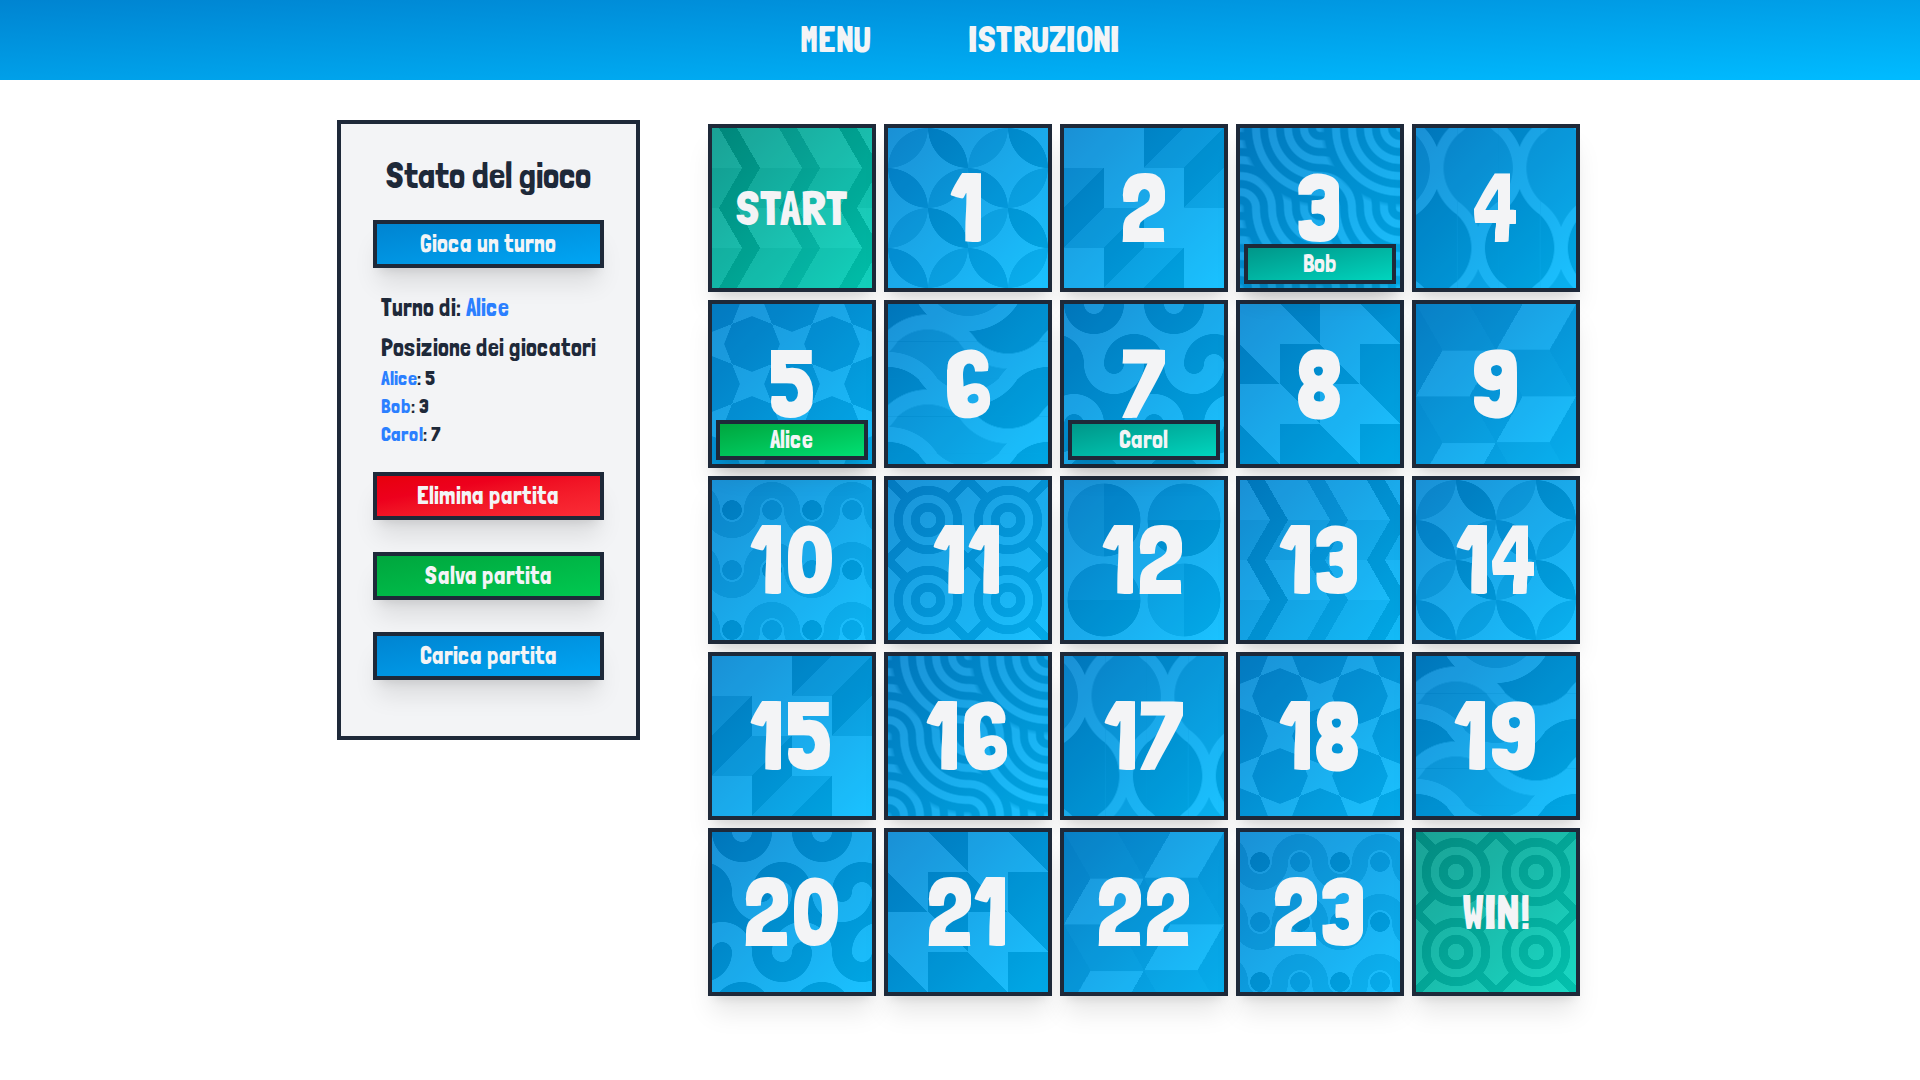
\includegraphics[width=\textwidth]{immagini/screenshots/game-board}
    \caption{Schermata di gioco: tabellone, barra laterale e dado.}
    \label{fig:game-board}
\end{figure}

\section{Architettura generale}

L'applicazione è distribuita su Vercel come progetto Next.js a pieno titolo: comprende una parte client-side (componenti React, CSS, JavaScript) e una parte server-side costituita dalle API Routes che supportano la modalità multi-dispositivo. Non è richiesta alcuna installazione: l'applicazione è accessibile da qualsiasi browser moderno su PC, laptop o tablet.

Nella modalità schermo singolo non vi è comunicazione di rete durante la partita: tutta la logica di gioco --- compresa la gestione dello stato, il salvataggio della partita e la generazione del tabellone --- risiede ed è eseguita nel browser dell'utente, con persistenza tramite \texttt{localStorage}. La modalità multi-dispositivo estende questa architettura con endpoint HTTP e uno store condiviso lato server, descritti nella sezione~\ref{sec:multi-dispositivo}.

\subsection{Evoluzione dall'architettura statica alla versione server-side}
\label{sec:evoluzione-architettura}

La prima versione dell'applicazione (\textbf{v1}, ultima release: 1.4.6) adottava la funzionalità di esportazione statica di Next.js: il processo di build produceva un insieme di file HTML, JavaScript e CSS distribuiti su GitHub Pages senza alcun server. Questa scelta garantiva semplicità di deploy e assenza di costi infrastrutturali, ma era incompatibile con le API Routes, rendendo impossibile implementare funzionalità che richiedessero stato condiviso tra dispositivi diversi.

La versione corrente (\textbf{v2}) abbandona l'esportazione statica e adotta Vercel come piattaforma di hosting. Le API Routes di Next.js sono ora abilitate e vengono eseguite come funzioni serverless al momento della richiesta. Lo stato delle sessioni è persistito su Upstash Redis, un servizio di key-value store accessibile tramite API HTTP, compatibile con l'ambiente serverless di Vercel. La versione v1 rimane accessibile all'indirizzo storico su GitHub Pages; la versione v2 è disponibile su Vercel all'indirizzo \texttt{https://tesi-nine.vercel.app/}.

\section{Storyboard: l'uso dell'applicazione da parte dell'educatore}
\label{sec:storyboard}

Questa sezione ripercorre passo per passo una sessione tipo dal punto di vista dell'educatore (o dello psicologo) che la conduce, dalla preparazione della partita alla chiusura. Per ogni fase si indicano che cosa fa l'educatore, che cosa fa l'applicazione e a quale scopo. Le singole schermate sono descritte nella sezione~\ref{sec:schermate}.

\subsection{Fase 1 --- Preparazione della partita}

La preparazione è comune alle due modalità ed è il momento in cui l'educatore adatta il gioco al gruppo (figure~\ref{fig:sb-prep} e~\ref{fig:sb-prep2}, tabella~\ref{tab:sb-prep}).

\begin{figure}[htbp]
    \centering
    \storypanel{mode-selection}{Passo 1: scelta della modalità.}{0.7\textwidth}

    \vspace{0.8em}

    \storypanel{home-single-filled}{Passi 2--5 e 7: configurazione (schermo singolo).}{0.7\textwidth}
    \caption{Preparazione della partita (1/2).}
    \label{fig:sb-prep}
\end{figure}

\begin{figure}[htbp]
    \centering
    \storypanel{home-multi-config}{Passi 3--5 e 7: configurazione (multi-dispositivo).}{0.7\textwidth}
    \caption{Preparazione della partita (2/2).}
    \label{fig:sb-prep2}
\end{figure}

\begingroup\small
\begin{longtable}{@{}c p{3.9cm} p{3.9cm} p{3.4cm}@{}}
\caption{Fase 1: preparazione della partita.}\label{tab:sb-prep}\\
\hline
\textbf{N.} & \textbf{L'educatore} & \textbf{L'applicazione} & \textbf{Finalità} \\ \hline
\endfirsthead
\hline
\textbf{N.} & \textbf{L'educatore} & \textbf{L'applicazione} & \textbf{Finalità} \\ \hline
\endhead
1 & Sceglie la modalità: schermo singolo o multi-dispositivo. & Mostra la selezione; ``Cambia modalità'' permette di tornare indietro. & Adattare la sessione agli spazi e al gruppo (sezione~\ref{sec:contesto}). \\ \hline
2 & Solo in schermo singolo: imposta numero di giocatori (2--10) e nomi. In multi-dispositivo i giocatori si registrano dallo smartphone. & Assegna un colore a ciascun giocatore. & Rendere ogni giocatore riconoscibile sul tabellone. \\ \hline
3 & Definisce la lunghezza del percorso (10--100 caselle). & Adegua la griglia del tabellone. & Regolare la durata della sessione. \\ \hline
4 & Sceglie le tipologie di caselle speciali e la loro percentuale. & Genera il tabellone con le sole tipologie scelte. & Orientare la sessione verso le competenze da esercitare, o escludere sfide non adatte al gruppo. \\ \hline
5 & Attiva o disattiva la Battaglia. & Se attiva, gestisce le collisioni tra pedine. & Dosare la componente competitiva. \\ \hline
6 & Facoltativo: apre la modalità avanzata e assegna a mano il tipo di ogni casella (figura~\ref{fig:advanced-mode}). & Sostituisce la distribuzione casuale. & Costruire un percorso su misura. \\ \hline
7 & Preme ``Inizia gioco''. & Mescola i mazzi e salva la configurazione nel \texttt{localStorage}. & Avviare la partita; la configurazione resta disponibile dopo un ricaricamento. \\ \hline
\end{longtable}
\endgroup

\subsection{Fase 2 --- Sessione a schermo singolo}

Tutti i partecipanti guardano lo stesso schermo. L'educatore conduce la partita e resta il riferimento per la valutazione delle sfide (figure~\ref{fig:sb-single} e~\ref{fig:sb-single2}, tabella~\ref{tab:sb-single}).

\begin{figure}[htbp]
    \centering
    \begin{tabular}{@{}p{0.46\textwidth}@{\hspace{1.5em}}p{0.46\textwidth}@{}}
    \shot{dice-roll}{Passo 1: lancio del dado.} &
    \shot{quiz-modal-answer}{Passi 3--4: sfida (Quiz) e registrazione dell'esito.} \\
    \end{tabular}
    \caption{Sessione a schermo singolo (1/2).}
    \label{fig:sb-single}
\end{figure}

\begin{figure}[htbp]
    \centering
    \begin{tabular}{@{}p{0.46\textwidth}@{\hspace{1.5em}}p{0.46\textwidth}@{}}
    \shot{skip-turn-modal}{Passo 4: turno saltato.} &
    \shot{end-game}{Passo 6: fine della partita.} \\
    \end{tabular}
    \caption{Sessione a schermo singolo (2/2).}
    \label{fig:sb-single2}
\end{figure}

\begingroup\small
\begin{longtable}{@{}c p{3.9cm} p{3.9cm} p{3.4cm}@{}}
\caption{Fase 2: sessione a schermo singolo.}\label{tab:sb-single}\\
\hline
\textbf{N.} & \textbf{L'educatore} & \textbf{L'applicazione} & \textbf{Finalità} \\ \hline
\endfirsthead
\hline
\textbf{N.} & \textbf{L'educatore} & \textbf{L'applicazione} & \textbf{Finalità} \\ \hline
\endhead
1 & Invita il giocatore di turno a premere il pulsante del dado. & Anima il lancio e sposta la pedina casella per casella. & Turni condivisi, senza dadi fisici. \\ \hline
2 & Osserva la casella raggiunta; se è normale il turno passa al giocatore successivo. & Aggiorna barra laterale e turno. & --- \\ \hline
3 & Se la casella è speciale, conduce la sfida mostrata nella finestra modale (figure~\ref{fig:modali-1}--\ref{fig:modali-2b}). & Estrae la carta dal mazzo corrispondente e la mostra a tutti. & Esercitare la competenza associata alla sfida (tabella~\ref{tab:sfide}). \\ \hline
4 & Valuta l'esito e lo registra. & Applica le conseguenze: avanzamento, retrocessione o salto del turno. & L'educatore resta il giudice della sfida. \\ \hline
5 & Se due pedine occupano la stessa casella e la Battaglia è attiva, guida la sfida a morra cinese. & Attiva la Battaglia e applica l'esito sul tabellone. & Competizione regolamentata. \\ \hline
6 & Alla partita conclusa proclama il vincitore. & Mostra la schermata di fine partita. & Gestire vittoria e sconfitta. \\ \hline
\end{longtable}
\endgroup

\subsection{Fase 3 --- Sessione multi-dispositivo}

Ogni giocatore usa il proprio smartphone, mentre il tabellone resta sullo schermo dell'educatore (figure~\ref{fig:sb-multi} e~\ref{fig:sb-multi2}, tabella~\ref{tab:sb-multi}). Le scelte tecniche che stanno dietro a questi passi sono descritte nella sezione~\ref{sec:multi-dispositivo}.

\begin{figure}[htbp]
    \centering
    \storypanel{multiplayer-lobby}{Passo 1: lobby con codice QR.}{0.46\textwidth}

    \vspace{0.8em}

    \begin{tabular}{@{}p{0.22\textwidth}@{\hspace{1.5em}}p{0.22\textwidth}@{}}
    \shot{multiplayer-join}{Passo 2: registrazione dal telefono.} &
    \shot{player-active-turn}{Passo 4: giocatore di turno.} \\
    \end{tabular}
    \caption{Sessione multi-dispositivo (1/2).}
    \label{fig:sb-multi}
\end{figure}

\begin{figure}[htbp]
    \centering
    \storypanel{multiplayer-board}{Passi 3--5: tabellone dell'educatore.}{0.46\textwidth}

    \vspace{0.8em}

    \begin{tabular}{@{}p{0.22\textwidth}@{\hspace{1.5em}}p{0.22\textwidth}@{}}
    \shot{player-waiting-turn}{Passo 4: gli altri giocatori.} &
    \shot{player-game-over}{Passo 6: fine partita.} \\
    \end{tabular}
    \caption{Sessione multi-dispositivo (2/2).}
    \label{fig:sb-multi2}
\end{figure}

\begingroup\small
\begin{longtable}{@{}c p{3.9cm} p{3.9cm} p{3.4cm}@{}}
\caption{Fase 3: sessione multi-dispositivo.}\label{tab:sb-multi}\\
\hline
\textbf{N.} & \textbf{L'educatore} & \textbf{L'applicazione} & \textbf{Finalità} \\ \hline
\endfirsthead
\hline
\textbf{N.} & \textbf{L'educatore} & \textbf{L'applicazione} & \textbf{Finalità} \\ \hline
\endhead
1 & Crea la sessione dalla configurazione e mostra il codice QR ai partecipanti. & Genera l'identificativo di sessione e il token dell'educatore; mostra la lobby. & Accesso dei giocatori senza digitare indirizzi. \\ \hline
2 & Attende che i giocatori inquadrino il QR e inseriscano il proprio nome. & Assegna a ciascuno un identificativo e aggiorna la lobby. & Ogni partecipante gioca dal proprio dispositivo. \\ \hline
3 & Preme ``Avvia partita''. & Porta tutti i dispositivi alla schermata di gioco. & --- \\ \hline
4 & Segue il tabellone; il giocatore di turno lancia il dado dal proprio smartphone. & Propaga il risultato a tutti; gli altri vedono chi è di turno. & Il tabellone resta il riferimento comune. \\ \hline
5 & Sulle caselle speciali supervisiona la sfida: mostra la risposta (Quiz), indica chi ha indovinato (Mimo) o registra l'esito. & Distribuisce la sfida ai dispositivi, in forma condivisa o privata (tabella~\ref{tab:sfide}). & Preservare l'elemento di sorpresa nelle sfide private. \\ \hline
6 & Conclude la partita. & Mostra il vincitore e il pulsante ``Dai un feedback!''. & Passare alla raccolta di feedback. \\ \hline
\end{longtable}
\endgroup

\subsection{Fase 4 --- Chiusura}

Al termine, o in caso di interruzione, l'educatore può:

\begin{itemize}
    \item riprendere la sessione in un secondo momento: la partita è conservata nel browser e può essere esportata come file JSON e ricaricata (sezione~\ref{sec:ripristino});
    \item invitare i partecipanti a compilare il modulo di feedback (sezione~\ref{sec:raccolta-feedback});
    \item consultare le risposte aggregate nella dashboard di analisi (sezione~\ref{sec:desc-feedback-dashboard}).
\end{itemize}

\section{Le schermate dell'applicazione}
\label{sec:schermate}

Questa sezione descrive le singole schermate incontrate nello storyboard. Se non diversamente indicato, gli screenshot riportati si riferiscono alla modalità a schermo singolo; le schermate proprie della modalità multi-dispositivo sono descritte nella sezione~\ref{sec:desc-multi-dispositivo}. La navigazione avviene tramite un header persistente che espone due elementi: un link diretto alla schermata delle istruzioni e un pulsante Menu che apre una finestra modale con i collegamenti a Nuova partita, Continua partita, Carica partita e Feedback.

\subsection{Schermata di gioco}

È la schermata principale, composta da tre aree:

\begin{itemize}
    \item \textbf{Tabellone} --- Griglia di caselle numerate, identificate visivamente per tipologia; le pedine si animano al momento dello spostamento.
    \item \textbf{Barra laterale} --- Mostra il giocatore attivo, il numero del round e le posizioni di tutti i giocatori.
    \item \textbf{Dado e modali} --- Un pulsante permette al giocatore attivo di lanciare il dado; se la casella di arrivo è speciale, si apre la finestra modale corrispondente alla sfida.
\end{itemize}

Le sfide attivabili sono quelle descritte nella sezione~\ref{sec:lcdi}. Ciascuna viene presentata attraverso una finestra modale sovrapposta al tabellone al momento dell'attivazione, come mostrato, per la modalità a schermo singolo, nelle figure~\ref{fig:modali-1}--\ref{fig:modali-2b}; la tabella~\ref{tab:sfide} riassume come è gestita nelle due modalità.

\begin{figure}[htbp]
    \centering
    \begin{tabular}{@{}p{0.46\textwidth}@{\hspace{1.5em}}p{0.46\textwidth}@{}}
    \shotS{mime-modal-topic}{Mimo.} &
    \shotS{quiz-modal-answer}{Quiz.} \\
    \end{tabular}
    \caption{Finestre modali delle sfide, modalità a schermo singolo (1/4): Mimo, Quiz.}
    \label{fig:modali-1}
\end{figure}

\begin{figure}[htbp]
    \centering
    \begin{tabular}{@{}p{0.46\textwidth}@{\hspace{1.5em}}p{0.46\textwidth}@{}}
    \shotS{backwrite-modal-word}{Parole alle spalle.} &
    \shotS{dictation-draw-modal-image}{Disegno dettato.} \\
    \end{tabular}
    \caption{Finestre modali delle sfide, modalità a schermo singolo (2/4): Parole alle spalle, Disegno dettato.}
    \label{fig:modali-1b}
\end{figure}

\begin{figure}[htbp]
    \centering
    \begin{tabular}{@{}p{0.46\textwidth}@{\hspace{1.5em}}p{0.46\textwidth}@{}}
    \shotS{music-emotion-modal}{Emozioni in musica.} &
    \shotS{face-emotion-modal-answer}{Indovina l'emozione.} \\
    \end{tabular}
    \caption{Finestre modali delle sfide, modalità a schermo singolo (3/4): Emozioni in musica, Indovina l'emozione.}
    \label{fig:modali-2}
\end{figure}

\begin{figure}[htbp]
    \centering
    \begin{tabular}{@{}p{0.46\textwidth}@{\hspace{1.5em}}p{0.46\textwidth}@{}}
    \shotS{what-would-you-do-modal}{Cosa faresti se\ldots} &
    \shotS{physical-test-modal}{Test fisico.} \\
    \end{tabular}
    \caption{Finestre modali delle sfide, modalità a schermo singolo (4/4): Cosa faresti se\ldots, Test fisico.}
    \label{fig:modali-2b}
\end{figure}

Nella modalità schermo singolo ogni sfida compare nella finestra modale visibile a tutti e l'educatore ne registra sempre l'esito. Nella modalità multi-dispositivo la visibilità dipende dalla sfida, come riassunto nella tabella~\ref{tab:sfide}.

\begingroup\small
\begin{longtable}{@{}p{3.6cm} p{4.4cm} p{5.0cm}@{}}
\caption{Gestione delle sfide nella modalità multi-dispositivo.}\label{tab:sfide}\\
\hline
\textbf{Sfida} & \textbf{Visibilità del contenuto} & \textbf{Esito} \\ \hline
\endfirsthead
\hline
\textbf{Sfida} & \textbf{Visibilità del contenuto} & \textbf{Esito} \\ \hline
\endhead
Quiz & Condivisa: la domanda è visibile a tutti, la risposta solo sul tabellone. & L'educatore mostra la risposta e registra successo o insuccesso. \\ \hline
Mimo & Privata: il tema compare solo sul telefono del giocatore attivo. & L'educatore indica quale giocatore ha indovinato, che riceve il beneficio. \\ \hline
Parole alle spalle, Disegno dettato & Privata: la parola o il disegno compaiono solo sul telefono del giocatore attivo, che sceglie il compagno destinatario. & Se la sfida riesce, entrambi avanzano di una casella. \\ \hline
Indovina l'emozione, Film, Emozioni in musica, Test fisico, Cosa faresti se\ldots & Condivisa: visibile a tutti. & L'educatore registra l'esito al termine. \\ \hline
Battaglia & Nessun contenuto: la morra cinese si svolge dal vivo e sul tabellone compaiono solo i nomi dei due giocatori. & L'educatore indica il vincitore; il server aggiorna le posizioni. \\ \hline
Caselle movimento & Nessuna sfida. & Applicate in automatico. \\ \hline
\end{longtable}
\endgroup


\subsection{Menu di navigazione}

Il menu è accessibile in qualsiasi momento tramite il pulsante \textbf{MENU} nell'header, indipendentemente dalla schermata corrente.
L'apertura sovrappone una finestra modale al contenuto sottostante senza interrompere lo stato della partita.

Il menu espone quattro collegamenti:
\begin{itemize}
    \item \textbf{Continua partita} --- reindirizza alla schermata di gioco, riprendendo la sessione in corso.
    \item \textbf{Nuova partita} --- reindirizza alla schermata Home per configurare una partita da zero.
    \item \textbf{Carica partita} --- reindirizza alla schermata Ripristina partita.
    \item \textbf{Dai un feedback!} --- reindirizza alla schermata Feedback.
\end{itemize}

Una sezione dedicata alle impostazioni audio consente di abilitare o disabilitare, tramite due caselle di spunta indipendenti, gli \textbf{effetti sonori} e gli \textbf{annunci vocali} dell'applicazione; la modifica è immediata e persistente per tutta la sessione. Gli annunci vocali --- disattivati di default --- leggono ad alta voce l'esito di ogni turno, il salto turno e la vittoria finale, offrendo un canale uditivo che rinforza le informazioni già mostrate a schermo: un supporto utile in particolare per chi fatica a seguire simultaneamente più stimoli visivi.

\begin{figure}[htbp]
    \centering
    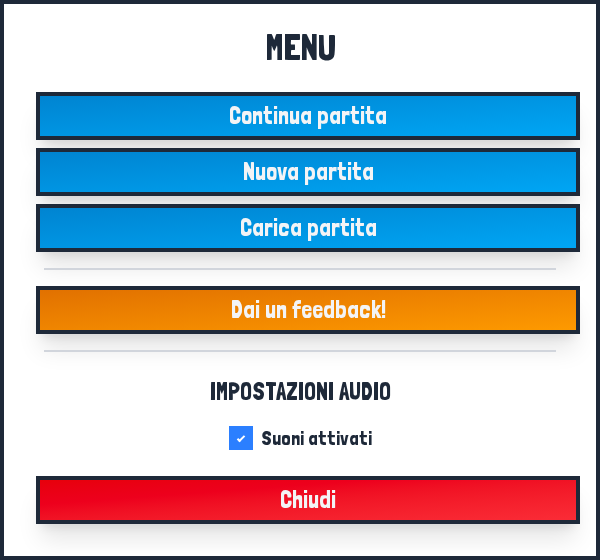
\includegraphics[width=\textwidth]{immagini/screenshots/menu}
    \caption{Menu di navigazione: collegamenti alle schermate principali e controllo audio.}
    \label{fig:menu}
\end{figure}

\subsection{Schermata Istruzioni}

Presenta le regole del gioco strutturate in sezioni (introduzione, configurazione, svolgimento del turno, caselle speciali, fine della partita), navigabili tramite un indice interno con link di ancoraggio.
Ogni sezione è corredata da video dimostrativi che mostrano l'applicazione in funzione nei principali scenari di gioco.
La schermata è raggiungibile direttamente dall'header in qualsiasi momento, senza perdere lo stato della partita in corso.

\subsection{Schermata Modalità avanzata}

Consente di assegnare manualmente il tipo a ogni singola casella del tabellone, sostituendo la distribuzione casuale.
L'interfaccia presenta un elenco scorrevole di tutte le caselle: ciascuna è identificata da un badge numerico il cui colore riflette il tipo attualmente assegnato.
La prima e l'ultima casella (Start e Fine) sono bloccate e non modificabili.
Per ogni casella intermedia è disponibile un menu a tendina con tutte le tipologie disponibili; selezionando il tipo \textit{movimento} compare un campo numerico aggiuntivo per specificare il numero di caselle di avanzamento o retrocessione (da $-5$ a $+5$).
I pulsanti in fondo alla schermata permettono di azzerare la configurazione, applicarla tornando alla schermata principale o annullare le modifiche.

\begin{figure}[htbp]
    \centering
    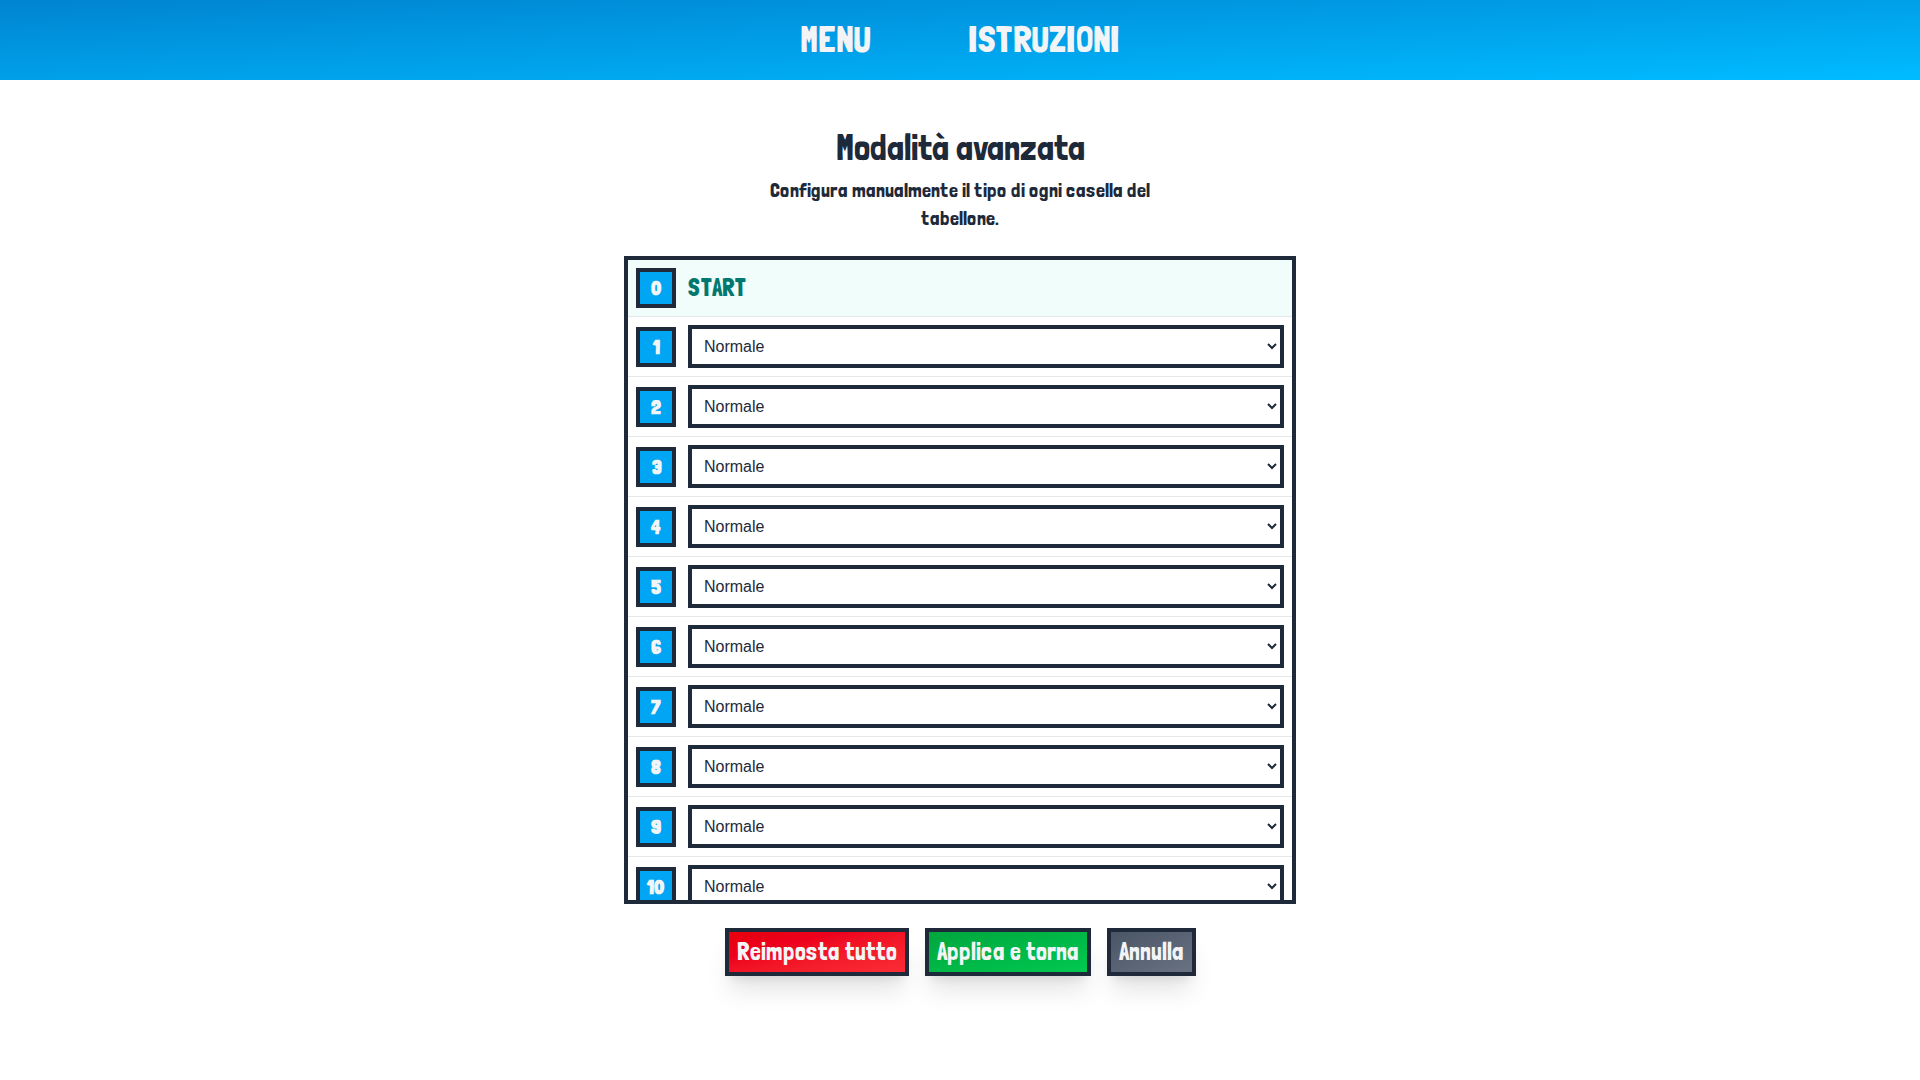
\includegraphics[width=\textwidth]{immagini/screenshots/advanced-mode}
    \caption{Schermata modalità avanzata: assegnazione manuale del tipo a ogni casella del tabellone.}
    \label{fig:advanced-mode}
\end{figure}

\subsection{Salvataggio e ripristino della partita}
\label{sec:ripristino}

Lo stato completo della partita (posizioni delle pedine, turno corrente, stato dei mazzi) è serializzabile in formato JSON ed esportabile come file. La schermata di ripristino consente di riprendere una sessione interrotta attraverso due modalità distinte.
La prima permette di caricare un file JSON esportato in precedenza: l'utente seleziona il file dal proprio dispositivo e avvia il ripristino; il sistema valida il contenuto e, in caso di file non valido, mostra un messaggio di errore.
La seconda modalità è disponibile quando il browser ha conservato automaticamente una partita nel \texttt{localStorage}: in tal caso compare un pulsante aggiuntivo per riprendere la sessione senza bisogno di alcun file.
In entrambi i casi, al termine del ripristino l'utente viene reindirizzato direttamente alla schermata di gioco.

\subsection{Schermata Feedback}

Il modulo, compilato al termine delle sessioni da docenti e alunni del CFPIL, raccoglie i dati di base del compilatore, il questionario standardizzato \textit{System Usability Scale} (SUS)~\cite{brooke1996sus}, alcune valutazioni numeriche e tre campi di testo libero; i campi sono elencati nella sezione~\ref{sec:raccolta-feedback}.
Le risposte, corredate dal numero di versione dell'applicazione al momento dell'invio, sono trasmesse all'endpoint interno \texttt{/api/feedback} e archiviate su Redis per analisi successive; un endpoint protetto da chiave segreta consente di esportare le risposte raccolte.

\subsection{Dashboard di analisi dei feedback}
\label{sec:desc-feedback-dashboard}

La schermata \texttt{/admin/feedback}, protetta dalla stessa chiave segreta dell'endpoint di esportazione, presenta in forma sintetica le risposte raccolte dal modulo Feedback.
La pagina interroga \texttt{/api/feedback} e calcola lato client il punteggio SUS medio secondo la formula standard~\cite{brooke1996sus}, mostrandolo insieme a un grado qualitativo.
Seguono le medie delle valutazioni numeriche e quattro grafici a barre con la distribuzione dei compilatori per ruolo, esperienza di gioco, identificazione neurodivergente e versione dell'applicazione: ciascuna barra è cliccabile e applica un filtro che ricalcola tutte le metriche della pagina sul sottoinsieme selezionato (i filtri sono cumulabili e removibili singolarmente). Il filtro per versione permette, ad esempio, di isolare i feedback raccolti dopo un rilascio specifico. L'elenco dei commenti liberi chiude la pagina.

\begin{figure}[htbp]
    \centering
    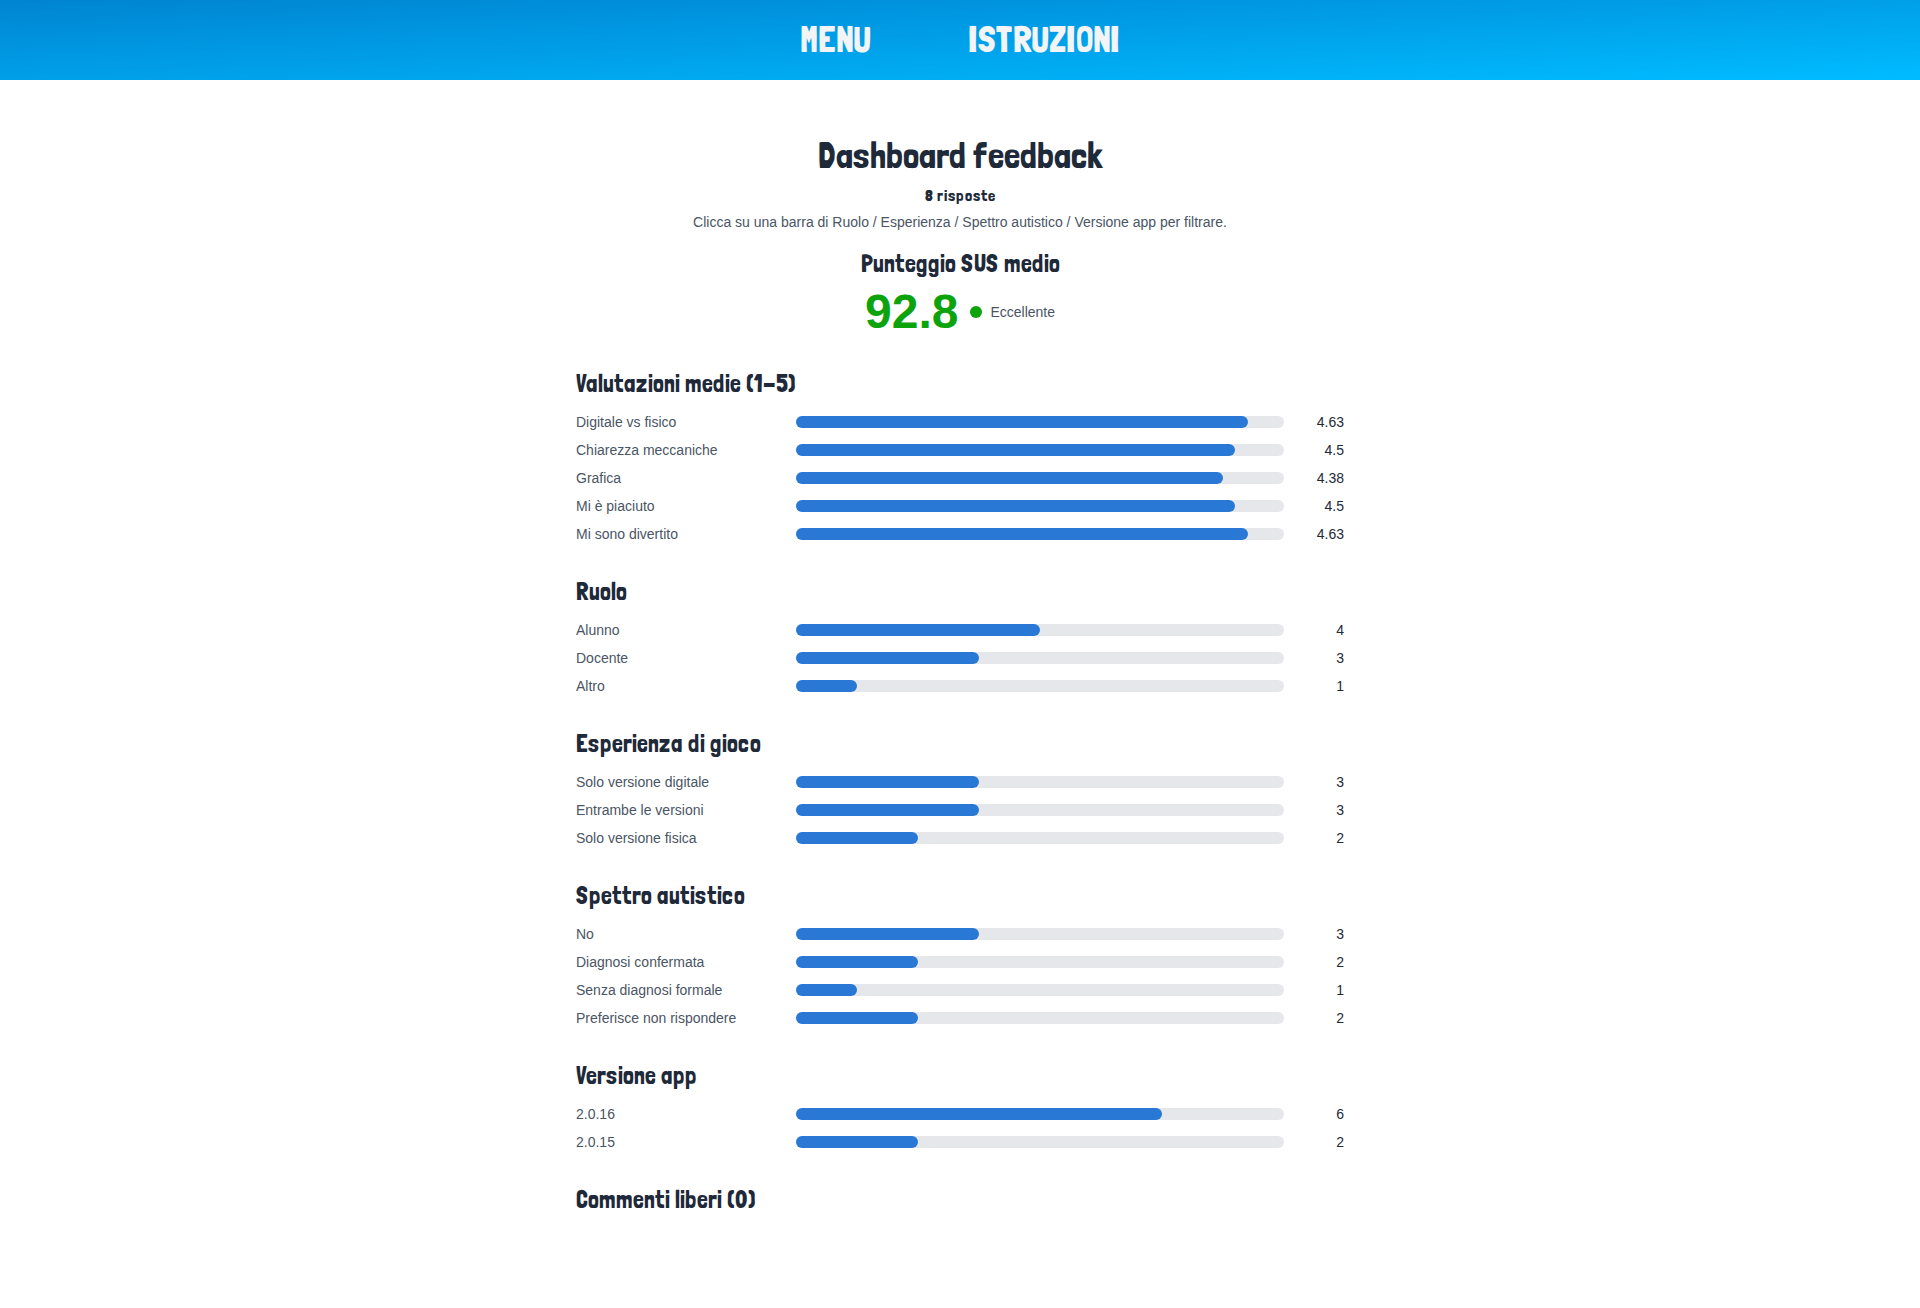
\includegraphics[width=\textwidth]{immagini/screenshots/feedback-dashboard}
    \caption{Dashboard di analisi dei feedback: punteggio SUS medio, valutazioni e distribuzione dei compilatori per categoria.}
    \label{fig:feedback-dashboard}
\end{figure}

\subsection{Modalità multi-dispositivo}
\label{sec:desc-multi-dispositivo}

Le schermate specifiche di questa modalità --- lobby con codice QR, pagina di registrazione e schermata personale del giocatore --- compaiono nello storyboard (figure~\ref{fig:sb-multi} e~\ref{fig:sb-multi2}).

Le sfide speciali si comportano diversamente a seconda della tipologia: per alcune il contenuto è \textbf{condiviso} e compare identico sul tabellone e sullo smartphone del giocatore attivo; per altre è \textbf{privato} e il tema resta visibile solo sul dispositivo di chi deve eseguirlo, mentre l'host vede unicamente i nomi dei giocatori coinvolti, preservando l'elemento a sorpresa.

\begin{figure}[htbp]
    \centering
    \begin{tabular}{@{}p{0.58\textwidth}@{\hspace{1.5em}}p{0.20\textwidth}@{}}
    \shotH{multiplayer-quiz-host}{Tabellone dell'educatore: domanda visibile, con pulsante per rivelare la risposta corretta.}{133pt} &
    \shotH{multiplayer-quiz-player}{Smartphone del giocatore: stessa domanda, in attesa del giudizio dell'educatore.}{133pt} \\
    \end{tabular}
    \caption{Sfida condivisa (Quiz): la domanda compare identica su entrambi gli schermi, ma la risposta resta visibile solo sul tabellone.}
    \label{fig:multiplayer-quiz}
\end{figure}

\begin{figure}[htbp]
    \centering
    \begin{tabular}{@{}p{0.58\textwidth}@{\hspace{1.5em}}p{0.20\textwidth}@{}}
    \shotH{multiplayer-physical-test-host}{Tabellone dell'educatore.}{133pt} &
    \shotH{multiplayer-physical-test-player}{Smartphone del giocatore.}{133pt} \\
    \end{tabular}
    \caption{Sfida condivisa (Test fisico): il contenuto compare identico su entrambi gli schermi.}
    \label{fig:multiplayer-physical-test}
\end{figure}

\begin{figure}[htbp]
    \centering
    \begin{tabular}{@{}p{0.58\textwidth}@{\hspace{1.5em}}p{0.20\textwidth}@{}}
    \shotH{multiplayer-dictation-draw-host}{Tabellone dell'educatore: nessun dettaglio della sfida è visibile, solo i nomi dei giocatori coinvolti.}{133pt} &
    \shotH{multiplayer-dictation-draw-player}{Smartphone del giocatore che descrive: tema e immagine di riferimento.}{133pt} \\
    \end{tabular}
    \caption{Sfida privata (Disegno dettato): il tema è visibile solo sul dispositivo del giocatore attivo.}
    \label{fig:multiplayer-dictation-draw}
\end{figure}

\begin{figure}[htbp]
    \centering
    \begin{tabular}{@{}p{0.58\textwidth}@{\hspace{1.5em}}p{0.20\textwidth}@{}}
    \shotH{multiplayer-mime-host}{Tabellone dell'educatore: il mimo da eseguire è nascosto, pronto per essere rivelato su richiesta.}{133pt} &
    \shotH{multiplayer-mime-player}{Smartphone del giocatore che mima: la parola o frase da mimare.}{133pt} \\
    \end{tabular}
    \caption{Sfida privata (Mimo) nella modalità multi-dispositivo.}
    \label{fig:multiplayer-mime}
\end{figure}

Per le sfide più dinamiche e fisiche (Mimo, Test fisico), la parte digitale si limita a distribuire il tema e a raccogliere l'esito: l'esecuzione vera e propria avviene fisicamente in aula ed è quindi meglio documentata con un video piuttosto che con uno screenshot statico.

L'architettura tecnica che supporta questa modalità è descritta nella sezione~\ref{sec:multi-dispositivo}.

\section{Architettura dei moduli}

Nella modalità schermo singolo, l'applicazione segue un'architettura a tre strati con separazione netta tra logica di dominio, gestione dello stato e presentazione, interamente eseguita nel browser. La modalità multi-dispositivo, descritta nella sezione~\ref{sec:multi-dispositivo}, sposta l'esecuzione autoritativa del Domain Model lato server e riduce Zustand, sul lato client, a un ruolo più marginale:

\begin{table}[h]
    \centering
    \begin{tabular}{|l|l|}
    \hline
    \textbf{Strato} & \textbf{Modulo} \\ \hline
    Presentation Layer     & Componenti React (\texttt{src/app/}) \\ \hline
    State Management Layer & Store Zustand (\texttt{src/store/}) \\ \hline
    Domain Model Layer     & Logica di gioco (\texttt{src/model/}) \\ \hline
    \end{tabular}
    \caption{Architettura a strati dell'applicazione (modalità schermo singolo).}
    \label{tab:architettura}
\end{table}

Questa separazione consente di testare la logica di gioco indipendentemente dall'interfaccia e di aggiornare i componenti visivi senza modificare le regole di gioco.

\subsection{Domain Model}
\label{sec:domain-model}

Il domain model contiene tutta la logica di gioco, completamente slegata da React e dal browser.
La classe \texttt{Game} è l'orchestratore principale: mantiene i riferimenti a tutti i sottocomponenti (tabellone, giocatori, dado, mazzi, manager) ed espone i metodi pubblici che il layer di stato chiama per far avanzare la partita.
Il metodo \texttt{playTurn()} esegue un turno completo --- lancio del dado, spostamento della pedina, elaborazione della casella --- e restituisce il tipo di azione da mostrare all'utente.
I metodi \texttt{toJSON()} e \texttt{fromJSON()} gestiscono la serializzazione dello stato per il salvataggio su file.

Ogni aspetto della partita è delegato a un manager specializzato:

\begin{itemize}
    \item \texttt{TurnManager} --- traccia il turno corrente, il round e il giocatore attivo;
    \item \texttt{MovementManager} --- sposta le pedine, gestisce bonus/malus di movimento e collisioni;
    \item \texttt{GameStateManager} --- verifica la condizione di vittoria;
    \item \texttt{SpecialSquareProcessor} --- determina quale azione speciale si attiva su una casella;
    \item \texttt{BattleManager} e i manager di ogni tipologia di sfida (es. \texttt{MimeManager}, \texttt{QuizManager}) --- applicano gli effetti dell'esito di ciascuna sfida.
\end{itemize}

Le caselle del tabellone sono modellate come classi distinte (es. \texttt{MimeSquare}, \texttt{QuizSquare}) che estendono la classe base \texttt{Square} e sono ricostruite tramite il pattern Builder al momento del ripristino di una partita salvata.

Ogni tipologia di casella speciale dispone di un mazzo di carte dedicato (es. \texttt{MimeDeck}, \texttt{QuizDeck}), mescolato all'inizio della partita e consumato in sequenza per garantire varietà e non ripetizione dei contenuti nella stessa sessione.

Il mazzo della sfida ``Indovina l'emozione'' (\texttt{FaceEmotionDeck}) utilizza fotografie tratte da FACES, un database open di volti che esprimono emozioni di base (felicità, rabbia, tristezza, paura, disgusto, neutralità), sviluppato dal Max Planck Institute for Human Development \cite{ebner2010faces}. A differenza delle illustrazioni disegnate usate per le altre sfide, l'impiego di volti fotografici reali e validati scientificamente rende più realistico e trasferibile l'esercizio di riconoscimento delle espressioni facciali.

Per ciascuna espressione non neutra è disponibile anche un'animazione di transizione (\textit{face morphing}) dall'espressione neutra a quella emotiva, generata automaticamente a partire dalle coppie di fotografie dello stesso soggetto. Uno script Python (\texttt{scripts/face\_morph.py}, eseguibile con \texttt{make face-morph}) rileva i 478 punti di riferimento del volto con il modello \textit{Face Landmarker} di MediaPipe, li triangola con la triangolazione di Delaunay e deforma ciascun triangolo in modo progressivo, miscelando i due scatti con una dissolvenza incrociata. La trasformazione è applicata solo all'interno di una maschera sfumata attorno al volto: sfondo e vestiario si spostano leggermente da uno scatto all'altro e, se deformati, mostrerebbero artefatti evidenti. Il risultato è un insieme di 60 gif (cinque espressioni, sei soggetti, due versioni di scatto), nominate come le fotografie di origine con il suffisso \texttt{\_morph}. Nell'interfaccia l'uso dell'animazione è una scelta esplicita, tramite l'opzione ``Animato''/``Non animato'' (disattivata di default), memorizzata in \texttt{localStorage} da uno store Zustand dedicato (\texttt{useFaceEmotionStore}). Il componente \texttt{FaceEmotionImage} che la gestisce è condiviso dalla finestra modale a schermo singolo, dall'\textit{overlay} dell'educatore e dalla schermata del giocatore di turno; se la gif non è disponibile, ripiega sulla fotografia statica.

La generazione procede, per ciascuna coppia (fotografia neutra, fotografia con espressione) dello stesso soggetto e della stessa versione di scatto, nei passi seguenti:
\begin{enumerate}
    \item le due fotografie, di circa 3500~px di larghezza, sono ridimensionate a 480~px di larghezza per contenere il peso della gif;
    \item su ciascuna sono rilevati i 478 punti di riferimento, ai quali si aggiungono otto punti fissi sul bordo dell'immagine (angoli e punti medi dei lati), in modo che la triangolazione copra l'intero fotogramma;
    \item la triangolazione di Delaunay è calcolata sulla media delle posizioni dei punti nelle due fotografie e resta la stessa per tutti i fotogrammi;
    \item per ogni fotogramma intermedio, con un parametro di avanzamento $\alpha$ tra 0 e 1, ciascun punto è portato nella posizione interpolata linearmente tra le due fotografie, i triangoli di entrambe le immagini sono deformati con una trasformazione affine verso tale posizione e i due risultati sono miscelati con pesi $1-\alpha$ e $\alpha$; $\alpha$ segue una curva \textit{ease-in/ease-out}, così che la transizione acceleri e rallenti gradualmente;
    \item il fotogramma finale è composto dentro la maschera del volto (inviluppo convesso dei punti del viso, sfumato con un filtro gaussiano con nucleo di 31~px), mentre l'esterno è preso invariato dalla fotografia neutra.
\end{enumerate}
La sequenza comprende 21 fotogrammi di transizione, una pausa di 6 fotogrammi sul volto neutro e sull'espressione, e il percorso inverso fino al neutro; la riproduzione è a 15 fotogrammi al secondo, in ciclo continuo.

Il mazzo della sfida ``Film'' (\texttt{FilmDeck}) contiene cinque scene, una per ciascuna emozione di base della sfida precedente esclusa la neutralità (felicità, rabbia, tristezza, disgusto, paura). La casella segue la stessa struttura delle altre sfide di riconoscimento delle emozioni: una \texttt{FilmSquare} esegue un comando che pesca una carta dal mazzo e restituisce un oggetto \texttt{Film}, la cui risoluzione è affidata a un \texttt{FilmManager}. Ogni carta associa l'emozione corretta a un file video servito dall'applicazione (cartella \texttt{public/videos}), in formato H.264 con audio AAC, risoluzione 852$\times$480 e durata compresa tra circa 17 e 24 secondi. Poiché il mazzo ha solo cinque carte e viene rimescolato una volta esaurito, nelle partite lunghe le scene si ripetono.

A differenza delle fotografie, la scena è un contenuto con voce e musica. Il componente \texttt{FilmVideo} usa il lettore nativo del browser, con i comandi visibili e senza avvio automatico, così che la riproduzione parta solo per scelta dell'utente e possa essere ripetuta; non sono disponibili sottotitoli. Il giocatore guarda la scena e indica l'emozione; l'educatore mostra la risposta con il pulsante ``Mostra risposta'' e registra l'esito. Se la risposta è corretta il giocatore avanza di una casella, altrimenti salta il turno successivo, come in ``Indovina l'emozione''.

\subsection{State Management}

Lo stato globale è gestito con Zustand, suddiviso in tre store indipendenti persistiti in \texttt{localStorage}:

\begin{itemize}
    \item \texttt{game-store} --- stato della partita in corso: istanza serializzata di \texttt{Game}, risultato del dado, tipo di azione corrente, stato delle finestre modali;
    \item \texttt{config-store} --- configurazione della partita: nomi e numero dei giocatori, numero di caselle, tipologie e percentuale di caselle speciali;
    \item \texttt{sound-store} --- preferenze dell'utente riguardo agli effetti sonori e agli annunci vocali.
\end{itemize}

Questa descrizione vale per intero nella modalità schermo singolo, dove \texttt{game-store} è l'unica fonte di verità e le sue azioni (\texttt{playTurn()}, \texttt{resolve*()}) sono l'unico punto d'ingresso per far avanzare la partita.
Nella modalità multi-dispositivo lo stato autoritativo risiede invece sul server (sezione~\ref{sec:multi-dispositivo-stato-client}): sulla pagina host \texttt{game-store} viene reidratato in sola lettura dallo snapshot ricevuto via \textit{polling} (\texttt{Game.fromJSON(session.gameState)}) e serve solo a renderizzare il tabellone, mentre le azioni dell'utente --- avvio partita, risoluzione delle sfide, lancio del dado --- vengono inviate direttamente alle API Routes tramite \texttt{fetch()}, bypassando le azioni dello store. Le pagine del giocatore (\texttt{app/player/}) e di accesso (\texttt{app/join/}) non usano Zustand: si affidano solo a \texttt{useState} locale e all'hook di \textit{polling} \texttt{useSessionPolling}.

\subsection{Presentation Layer}

Il presentation layer comprende sia le pagine che i componenti React.
In Next.js le pagine (\texttt{page.tsx}) sono esse stesse componenti: la distinzione è strutturale --- determinano il routing --- ma non concettuale.

Le pagine dell'applicazione sono:

\begin{itemize}
    \item \texttt{app/page.tsx} --- schermata di selezione modalità e configurazione della partita;
    \item \texttt{app/game/page.tsx} --- schermata principale di gioco (modalità schermo singolo);
    \item \texttt{app/multiplayer/page.tsx} --- lobby per la modalità multi-dispositivo (creazione sessione e QR code);
    \item \texttt{app/\allowbreak multiplayer/\allowbreak[sessionId]/\allowbreak page.tsx} --- tabellone host per la sessione multi-dispositivo;
    \item \texttt{app/\allowbreak player/\allowbreak[sessionId]/\allowbreak[playerId]/\allowbreak page.tsx} --- schermata del giocatore sullo smartphone;
    \item \texttt{app/\allowbreak join/\allowbreak[sessionId]/\allowbreak page.tsx} --- pagina di accesso tramite QR code, reindirizza alla registrazione;
    \item \texttt{app/instructions/page.tsx} --- istruzioni di gioco con video dimostrativi;
    \item \texttt{app/advanced-mode/page.tsx} --- configurazione avanzata del tabellone;
    \item \texttt{app/restore-game/page.tsx} --- ripristino partita da file;
    \item \texttt{app/feedback/page.tsx} --- modulo di feedback;
    \item \texttt{app/admin/feedback/page.tsx} --- dashboard di analisi dei feedback raccolti.
\end{itemize}

I componenti principali dell'interfaccia sono:

\begin{itemize}
    \item \texttt{board.tsx} --- tabellone come griglia CSS con numero di colonne variabile in base alla dimensione;
    \item \texttt{square.tsx} --- singola casella con numero, tipo visivo e pedine presenti;
    \item \texttt{pawn.tsx} --- pedina con colore assegnato e animazione al momento dello spostamento;
    \item \texttt{dice.tsx} --- dado con animazione al momento del lancio;
    \item \texttt{left-bar.tsx} --- barra laterale con turno attivo, round corrente e classifica;
    \item \texttt{turn-result-modal.tsx} --- finestra modale delegata a un sottocomponente specifico per ogni tipo di sfida.
\end{itemize}

I componenti primitivi riutilizzabili (\texttt{Button}, \texttt{Input}, \texttt{Label}, \texttt{Select}) sono sviluppati e documentati in isolamento tramite Storybook.

\section{Scelte implementative rilevanti}

\subsection{Il tipo \texttt{GameActionResult} e il Command Pattern}
\label{sec:command}

La comunicazione tra il domain model e il layer di stato avviene tramite il tipo \texttt{GameActionResult}, un oggetto TypeScript che \texttt{playTurn()} restituisce al termine di ogni turno.
Questa scelta riflette il \textit{Command Pattern}: invece di eseguire direttamente un'azione sull'interfaccia, il domain model produce un oggetto che \textit{descrive} l'azione da compiere, lasciando al chiamante la responsabilità di decidere come gestirla.

Il campo \texttt{type} è un'unione discriminata di stringhe letterali --- una per ogni tipologia di sfida più il valore \texttt{"none"} per i turni senza azione speciale. Il campo \texttt{data} trasporta i dati specifici dell'azione (ad esempio la carta estratta o i giocatori coinvolti in una battaglia). Lo store legge \texttt{type} per determinare quale finestra modale aprire, e \texttt{data} per popolarla con il contenuto corretto, senza che il domain model abbia alcuna dipendenza dall'interfaccia.
Il ciclo si chiude quando l'educatore registra l'esito della sfida: lo store chiama il corrispondente metodo \texttt{resolve*()} su \texttt{Game}, che applica le conseguenze sul tabellone e aggiorna lo stato della partita.

\begin{lstlisting}[language=TypeScript, caption={Tipo di ritorno di \texttt{playTurn()} (src/model/managers/types.ts)}]
export type GameActionResult = {
  type:
    | "battle" | "mime"    | "quiz"
    | "backwrite"          | "face-emotion"
    | "film"               | "music-emotion"
    | "physical-test"      | "what-would-you-do"
    | "dictation-draw"     | "none";
  data?: Battle | Mime | Quiz | BackWrite | FaceEmotion
       | Film | MusicEmotion | PhysicalTest
       | WhatWouldYouDo | DictationDraw;
  diceResult: number;
  actionType: string | null;
};
\end{lstlisting}

Il metodo \texttt{playTurn()} in \texttt{Game} sfrutta questo tipo per incapsulare l'intera logica del turno --- gestione del turno saltato, lancio del dado, movimento, rilevamento collisioni ed elaborazione della casella speciale --- restituendo un valore strutturato che il layer di stato consuma senza dover conoscere i dettagli interni.

\begin{lstlisting}[language=TypeScript, caption={Metodo \texttt{playTurn()} (src/model/game.ts)}]
playTurn(): GameActionResult {
  const currentPlayer = this.turnManager.getCurrentPlayer();

  if (currentPlayer.mustSkipTurn()) {
    this.turnManager.advanceTurn();
    return { type: "none", diceResult: 0, actionType: null };
  }

  const diceValue = this.dice.roll();
  const result = this.executePlayerTurn(currentPlayer, diceValue);
  this.turnManager.advanceTurn();

  return { ...result, diceResult: diceValue };
}
\end{lstlisting}

\subsection{Gestione dello stato con Zustand e persistenza}

Quanto segue descrive il funzionamento di \texttt{useGameStore} nella modalità schermo singolo, dove è l'unico punto di raccordo tra il domain model e l'interfaccia utente; il suo ruolo ridotto nella modalità multi-dispositivo è descritto nella sezione~\ref{sec:multi-dispositivo-stato-client}.
È definito tramite \texttt{create()} di Zustand, avvolto nel middleware \texttt{persist}, e si articola in due sezioni distinte: lo \textit{stato} e le \textit{azioni}.

La sezione di stato contiene due categorie di campi: quelli che riflettono la partita in corso (\texttt{game}, istanza della classe \texttt{Game}, e \texttt{gameData}, la sua rappresentazione JSON) e quelli che descrivono la situazione dell'interfaccia (\texttt{isModalOpen}, \texttt{isDiceModalOpen}, \texttt{diceResult}, \texttt{actionType}, \texttt{actionData} e altri).

Le azioni sono funzioni che i componenti React chiamano in risposta agli eventi dell'utente. La più importante è \texttt{playTurn()}: recupera l'istanza di \texttt{Game} dallo store, invoca il metodo omonimo del domain model, riceve il \texttt{GameActionResult} e aggiorna lo stato dell'interfaccia di conseguenza --- impostando il risultato del dado, il tipo di azione attiva e aprendo la finestra modale appropriata. Analogamente, ciascuna azione \texttt{resolve*()} delega la risoluzione al metodo corrispondente di \texttt{Game} e, al termine, aggiorna la serializzazione JSON della partita tramite \texttt{toJSON()}.

Il middleware \texttt{persist} sincronizza automaticamente lo store con il \texttt{localStorage} del browser. L'opzione \texttt{partialize} limita la persistenza al solo campo \texttt{gameData}: in questo modo lo stato della partita sopravvive al ricaricamento della pagina, mentre i campi transitori dell'interfaccia vengono reinizializzati ai valori di default.

\begin{lstlisting}[language=TypeScript, caption={Store di gioco con persistenza selettiva (src/store/game-store.ts)}]
export const useGameStore = create<GameStore>()(
  persist(
    (set, get) => ({
      game: null,
      gameData: null,
      isModalOpen: false,
      // ...altri campi UI...

      actions: {
        playTurn: () => {
          const { game } = get();
          if (!game) return;

          const { diceResult, actionType, data } = game.playTurn();
          // aggiorna lo stato UI in base al risultato...
        },
        // ...altri metodi...
      },
    }),
    {
      name: "game-store",
      partialize: (state) => ({
        gameData: state.gameData,
        hasSavedGame: !!state.gameData,
      }),
    },
  ),
);
\end{lstlisting}

\section{Design pattern utilizzati}

La progettazione dell'applicazione ha fatto uso di diversi design pattern consolidati \cite{gof1994}, applicati in modo coerente con le responsabilità dei moduli descritti nelle sezioni precedenti.

\subsection{Command Pattern}
Il pattern Command è applicato nella comunicazione tra il domain model e il layer di stato tramite il tipo \texttt{GameActionResult} (si veda la sezione~\ref{sec:command}): ogni turno produce un oggetto che \textit{descrive} l'azione da eseguire, disaccoppiando il mittente (il domain model) dal ricevente (lo store e l'interfaccia).

\subsection{Facade Pattern}
La classe \texttt{Game} agisce da \textit{Facade}: espone un'interfaccia semplice e coerente (\texttt{playTurn()}, \texttt{resolve*()}, \texttt{toJSON()}) nascondendo la complessità interna dei manager, dei mazzi e del tabellone. I componenti React e lo store non interagiscono mai direttamente con i sottosistemi interni.

\subsection{Builder Pattern}
Il modulo \texttt{square-builder.ts} implementa il pattern Builder per ricostruire le istanze delle caselle a partire dalla loro rappresentazione JSON durante il ripristino di una partita salvata. Poiché ogni tipologia di casella è una classe distinta, il Builder centralizza la logica di selezione del costruttore corretto in base al campo \texttt{type}.

\subsection{Observer Pattern}
Zustand adotta implicitamente il pattern Observer: i componenti React si \textit{sottoscrivono} a porzioni specifiche dello store tramite selettori, e vengono ri-renderizzati automaticamente solo quando i campi osservati cambiano. Questo evita aggiornamenti superflui dell'interfaccia e mantiene i componenti disaccoppiati dalla logica di aggiornamento dello stato.

\subsection{Manager Pattern}
La classe \texttt{Game} delega ciascuna responsabilità a un manager specializzato (sezione~\ref{sec:domain-model}).
Questo approccio --- talvolta chiamato \textit{Manager Pattern} o \textit{Specialist Pattern} --- consente di mantenere la classe \texttt{Game} snella e leggibile, concentrando ciascuna regola di gioco nel modulo che ne è responsabile, con benefici diretti sulla testabilità e sulla manutenibilità del codice.

\subsection{Model-View-Controller}
\label{sec:mvc}
Nella modalità schermo singolo, l'architettura a tre strati dell'applicazione rispecchia il pattern architetturale \textit{Model-View-Controller} (MVC): il Domain Model (\texttt{src/model/}) corrisponde al \textit{Model}, i componenti React (\texttt{src/app/}) alla \textit{View} e gli store Zustand (\texttt{src/store/}) al \textit{Controller}, che media le interazioni dell'utente verso il modello e propaga gli aggiornamenti di stato verso l'interfaccia. Nella modalità multi-dispositivo il ruolo di Controller passa alle API Routes, che ricevono le azioni via HTTP e le applicano a un'istanza di \texttt{Game} lato server (sezione~\ref{sec:multi-dispositivo-stato-client}); Zustand vi sopravvive solo come cache di rendering sulla pagina host.

\section{Modalità multi-dispositivo}
\label{sec:multi-dispositivo}

Di seguito si descrive l'architettura tecnica che supporta la modalità multi-dispositivo.

\subsection{Architettura delle sessioni}

La modalità multi-dispositivo richiede una componente \textit{server-side} per sincronizzare lo stato della partita tra i dispositivi dei giocatori. A tal fine, l'applicazione fa uso delle \textit{API Routes} di Next.js, che consentono di definire endpoint HTTP direttamente nel progetto senza la necessità di un server separato. La figura~\ref{fig:architettura-multi} riassume i componenti coinvolti e le comunicazioni descritte nel resto della sezione.

\begin{figure}[htbp]
    \centering
    \begin{tikzpicture}[
        box/.style={draw, rounded corners, align=center, font=\small, minimum height=1.1cm, inner sep=6pt},
        arr/.style={-{Stealth[length=6pt]}, thick},
        lbl/.style={font=\scriptsize, align=center},
        node distance=1.3cm and 1cm
    ]
        \node[box, minimum width=3cm] (host) {Host\\(tablet/PC dell'educatore)\\\texttt{/multiplayer/[id]}};
        \node[box, minimum width=2.8cm, right=1.4cm of host] (player) {Giocatore\\(smartphone)\\\texttt{/player/[id]/[pid]}};

        \node[box, minimum width=7.3cm, below=1.5cm of $(host)!0.5!(player)$] (api) {Vercel --- API Routes\\(funzioni serverless)};

        \node[box, minimum width=5.5cm, below=1.5cm of api] (redis) {Upstash Redis\\\texttt{SessionState}};

        \draw[arr] (host) -- (api) node[lbl, midway, left, xshift=-2pt] {long polling\\\texttt{GET /api/sessions/[id]}};
        \draw[arr] (player) -- (api) node[lbl, midway, right, xshift=2pt] {long polling\\+ \texttt{POST} azioni};
        \draw[arr, <->] (api) -- (redis) node[lbl, midway, right, xshift=2pt] {lettura/scrittura\\stato di sessione};
        \draw[arr, dashed] (host) to[bend left=18] node[lbl, midway, above, sloped] {codice QR / \texttt{join}} (player);
    \end{tikzpicture}
    \caption{Architettura della modalità multi-dispositivo: host e giocatori comunicano con le API Routes tramite \textit{long polling}, che leggono e scrivono lo stato di sessione su Redis; il giocatore si unisce inquadrando il codice QR mostrato dall'host.}
    \label{fig:architettura-multi}
\end{figure}

Lo stato di sessione è rappresentato da un oggetto \texttt{SessionState} che include l'elenco dei giocatori connessi, la fase corrente della partita, il turno attivo e gli esiti delle sfide. La persistenza di questo stato è gestita tramite un meccanismo a tre livelli, scelto in cascata in base all'ambiente di esecuzione:

\begin{enumerate}
    \item \textbf{Upstash Redis} --- in produzione, lo stato è memorizzato su Upstash Redis (descritto nel capitolo~\ref{cap:tecnologie}), tramite il client \texttt{@upstash/redis} configurato con le variabili di ambiente della piattaforma;
    \item \textbf{ioredis} --- in sviluppo locale con Redis disponibile, si utilizza il client \texttt{ioredis} per connettersi a un'istanza Redis locale;
    \item \textbf{Map in memoria} --- in assenza di Redis, lo stato è mantenuto in una \texttt{Map} JavaScript in memoria del processo Node.js, sufficiente per lo sviluppo locale su singola istanza.
\end{enumerate}

Questa struttura garantisce portabilità tra ambienti senza modifiche al codice applicativo: la selezione del livello appropriato avviene in fase di inizializzazione in base alle variabili di ambiente disponibili.

La creazione di una sessione avviene tramite una richiesta \texttt{POST} all'endpoint \texttt{/api/sessions}, che restituisce un identificatore di sessione (\texttt{sessionId}) e un \texttt{hostToken}, un token opaco conservato nel \texttt{localStorage} del dispositivo dell'educatore e allegato alle successive richieste privilegiate per autorizzarle.

\subsection{Connessione dei giocatori tramite QR code}

Una volta creata la sessione, l'applicazione genera un codice QR che i giocatori inquadrano con il proprio smartphone. Il codice QR contiene l'URL della pagina di accesso, che include il \texttt{sessionId} come parametro. Il giocatore inserisce il proprio nome e invia una richiesta \texttt{POST} all'endpoint \texttt{/api/sessions/[id]/join}, che registra il nuovo partecipante nella sessione e restituisce un \texttt{playerId} univoco.

Il giocatore viene quindi reindirizzato alla propria schermata di gioco, raggiungibile all'URL \texttt{/player/[sessionId]/[playerId]}. L'identità del giocatore è interamente codificata nell'URL: anche in caso di chiusura accidentale della scheda o di ricaricamento della pagina, il giocatore recupera il proprio stato semplicemente riaprendo lo stesso indirizzo.

\subsection{Stato lato client: il ruolo ridotto di Zustand}
\label{sec:multi-dispositivo-stato-client}

A differenza della modalità schermo singolo (sezione~\ref{sec:domain-model}), in modalità multi-dispositivo l'istanza di \texttt{Game} autoritativa vive lato server: le API Routes la ricostruiscono da \texttt{SessionState} tramite \texttt{Game.fromJSON()}, invocano su di essa i metodi del domain model e ne persistono il risultato su Redis. Il client non possiede quindi una copia mutabile della partita, ma solo lo snapshot pubblico ricevuto tramite \textit{long polling}.

Questo capovolge il ruolo di Zustand rispetto alla modalità schermo singolo:

\begin{itemize}
    \item sulla pagina host (\texttt{app/\allowbreak multiplayer/\allowbreak[sessionId]/\allowbreak page.tsx}), \texttt{game-store} viene reidratato in sola lettura a ogni aggiornamento del \textit{polling} (\texttt{gameStore.\allowbreak setGame(\allowbreak Game.\allowbreak fromJSON(\allowbreak session.\allowbreak gameState))}) e serve esclusivamente a renderizzare il tabellone; le azioni dell'educatore (avvio partita, risoluzione di una sfida, designazione di un vincitore) non passano per le azioni dello store ma vengono inviate come richieste \texttt{POST} dirette agli endpoint \texttt{/api/sessions/[id]/*};
    \item \emergencystretch=3em le pagine \texttt{app/\allowbreak player/\allowbreak[sessionId]/\allowbreak[playerId]/\allowbreak page.tsx} e \texttt{app/\allowbreak join/\allowbreak[sessionId]/\allowbreak page.tsx} non importano né \texttt{useGameStore} né \texttt{useConfigStore}: si basano unicamente su \texttt{useState} locale e sull'hook \texttt{useSessionPolling} (\texttt{src/\allowbreak lib/\allowbreak use-session-polling.ts}), che espone direttamente lo stato pubblico di sessione ricevuto dal server.
\end{itemize}

In sintesi, la tabella~\ref{tab:architettura} e la lettura MVC della sezione~\ref{sec:mvc} descrivono l'architettura della sola modalità schermo singolo; in modalità multi-dispositivo lo strato di gestione dello stato --- e con esso il ruolo di Controller --- si sposta alle API Routes lato server, mentre Zustand resta attivo, ridotto a cache di presentazione, solo sulla pagina host.

\subsection{Comunicazione in tempo reale tramite \textit{long polling}}

Per notificare i dispositivi dei giocatori degli aggiornamenti di stato senza l'uso di connessioni persistenti, la modalità multi-dispositivo adotta la tecnica del \textit{long polling}. Ogni dispositivo invia periodicamente una richiesta \texttt{GET} all'endpoint \texttt{/api/sessions/[id]}, passando come parametro il valore \texttt{updatedAt} dell'ultimo stato ricevuto. Il server, anziché rispondere immediatamente, mantiene la connessione aperta per un massimo di otto secondi, interrogando lo \textit{store} ogni trecento millisecondi; restituisce la risposta non appena rileva che il campo \texttt{updatedAt} dello stato corrente è più recente di quello del client, oppure allo scadere del \textit{timeout}.

Questo approccio riduce il numero di invocazioni delle \textit{serverless function} di circa cinque volte rispetto al \textit{polling} a intervallo fisso, un aspetto rilevante ai fini della compatibilità con il piano gratuito di Vercel, che impone limiti al numero di esecuzioni mensili. La scelta del \textit{long polling} in luogo dei WebSocket è motivata dalla stessa considerazione: il piano \textit{Hobby} di Vercel non supporta connessioni WebSocket persistenti, mentre le richieste HTTP di lunga durata sono gestite nativamente dalle \textit{serverless function}.

\subsection{Rilevamento dell'inattività}

Per evitare il consumo inutile di risorse in caso di dispositivi lasciati incustoditi, la modalità multi-dispositivo include un meccanismo di rilevamento dell'inattività. Il \textit{polling} viene sospeso automaticamente dopo trenta minuti di inattività del giocatore; sullo schermo compare un \textit{overlay} con il messaggio \textit{``Stai ancora giocando?''}, che invita l'utente a confermare la propria presenza. In assenza di interazione per ulteriori cinque minuti, il \textit{polling} si interrompe definitivamente. Qualsiasi interazione con il dispositivo --- un tocco sullo schermo, un'azione di gioco --- è sufficiente a riprendere il ciclo di aggiornamento.

\subsection{Svolgimento del turno in modalità multi-dispositivo}

Nel corso della partita, il flusso di ogni turno si svolge come segue:

\begin{enumerate}
    \item L'educatore avvia la partita premendo il pulsante \textbf{Avvia partita} dalla schermata di \textit{lobby}; tutti i dispositivi ricevono l'aggiornamento di stato e passano alla schermata di gioco.
    \item Quando è il proprio turno, il giocatore attivo lancia il dado dal proprio dispositivo; il risultato viene comunicato al server e propagato agli altri partecipanti. Sul proprio schermo, il giocatore attivo visualizza prima una schermata intermedia con il valore del dado e la casella raggiunta, e prosegue premendo il pulsante \textbf{Avanti} prima di accedere alla sfida o al turno successivo.
    \item Se la casella di arrivo non attiva alcuna sfida speciale, il turno termina e il controllo passa al giocatore successivo.
    \item Se la casella attiva una sfida, la gestione varia in base alla tipologia (tabella~\ref{tab:sfide}). Mentre la sfida è in corso, i giocatori non coinvolti visualizzano sul proprio dispositivo un'animazione (un'icona a forma di dado in rotazione) al posto di un semplice messaggio testuale, a indicare l'attesa dello svolgimento dell'azione da parte di un altro giocatore.
    \item Al termine di ogni sfida, l'educatore conferma l'esito sull'interfaccia; il server aggiorna lo stato della sessione e tutti i dispositivi ricevono la notifica dell'avanzamento.
\end{enumerate}

Al termine della partita, tutti i dispositivi visualizzano la schermata di fine gioco con il nome del vincitore; sui dispositivi dei singoli giocatori la schermata include anche il pulsante \textbf{Dai un feedback!}, che reindirizza alla schermata Feedback.

\subsection{Considerazioni sulla dimensione sociale}

L'introduzione della modalità multi-dispositivo modifica in modo rilevante la dinamica relazionale del gioco. Nella modalità schermo singolo tutti i partecipanti guardano lo stesso schermo: l'attenzione del gruppo converge su un punto fisico condiviso, favorendo quella che la letteratura indica come \textit{joint attention} --- un costrutto rilevante nell'intervento sull'ASD \cite{mesibov2005}. Le sfide si svolgono davanti a tutti, e l'interazione tra i giocatori è continua e visibile.

Nella modalità multi-dispositivo, invece, ciascun giocatore interagisce prevalentemente con il proprio schermo. Sebbene alcune sfide --- come Mimo e Test fisico --- mantengano una componente di interazione fisica diretta, l'attenzione tende a distribuirsi sui singoli dispositivi anziché convergere su un punto comune. Questa frammentazione potrebbe limitare, almeno parzialmente, la qualità dell'interazione faccia a faccia che costituisce uno dei vantaggi chiave del gioco da tavolo rispetto ai serious games individuali descritti dalla letteratura \cite{carneiro2024, atherton2021}.

Il vantaggio specifico della modalità multi-dispositivo risiede nell'accessibilità e nella gestione della segretezza: consente di giocare in contesti in cui non è disponibile uno schermo condiviso sufficientemente grande, e permette che per alcune sfide --- come Mimo e Disegno dettato --- il tema da rappresentare compaia esclusivamente sullo schermo del giocatore attivo, senza essere visibile agli altri prima che la sfida abbia inizio. La scelta tra le due modalità dipende pertanto dagli obiettivi dell'educatore: la modalità schermo singolo è preferibile quando l'obiettivo primario è stimolare la \textit{joint attention} e l'interazione faccia a faccia; la modalità multi-dispositivo è indicata quando si intende promuovere l'uso autonomo della tecnologia o quando non è disponibile un unico schermo condiviso di dimensioni adeguate.

%
%			CAPITOLO 5: Test
%

\chapter{Test}
\label{cap:test}

\section{Raccolta di feedback}
\label{sec:raccolta-feedback}

Al termine delle sessioni di utilizzo, i partecipanti del CFPIL di Varese sono stati invitati a compilare il modulo di feedback integrato nell'applicazione. Per ridurre il carico percettivo delle numerose domande, il modulo è organizzato come un percorso guidato a step (\emph{wizard}) suddiviso in quattro fasi --- informazioni di base, questionario SUS, valutazioni e domande aperte --- con avanzamento vincolato alla compilazione dei campi obbligatori di ciascuna fase. Il modulo raccoglie:

\begin{itemize}
    \item \textbf{nome};
    \item \textbf{ruolo} --- docente, alunno o altro;
    \item \textbf{esperienza pregressa con il gioco} --- versione fisica, digitale o entrambe;
    \item \textbf{modalità di gioco} --- schermo singolo o multischermo;
    \item \textbf{questionario SUS} --- 10 affermazioni standardizzate della \textit{System Usability Scale}~\cite{brooke1996sus}, ciascuna valutata in scala 1--5;
    \item \textbf{fedeltà della versione digitale rispetto a quella fisica} --- valutazione in scala 1--5, facoltativa;
    \item \textbf{chiarezza dei meccanismi di gioco} --- valutazione in scala 1--5;
    \item \textbf{grafica} --- valutazione in scala 1--5;
    \item \textbf{gradimento complessivo} --- valutazione in scala 1--5;
    \item \textbf{divertimento} --- valutazione in scala 1--5;
    \item \textbf{aspetti positivi};
    \item \textbf{aspetti negativi};
    \item \textbf{suggerimenti di miglioramento};
    \item \textbf{identificazione neurodivergente/autistica} --- facoltativa, utile per leggere i feedback anche in relazione a eventuali bisogni specifici;
    \item \textbf{versione dell'applicazione} --- registrata automaticamente al momento dell'invio.
\end{itemize}

Le risposte raccolte sono state analizzate tramite la dashboard descritta nel paragrafo~\ref{sec:desc-feedback-dashboard} (figura~\ref{fig:feedback-dashboard}), che calcola il punteggio SUS medio e la distribuzione delle valutazioni per categoria senza richiedere l'esportazione manuale dei dati.

%
%			CAPITOLO 6: Conclusioni e sviluppi futuri
% 

\chapter{Conclusioni}
\label{cap:conclusioni}

\section{Riepilogo del lavoro}

Questo elaborato ha descritto la progettazione e lo sviluppo di una versione digitale del gioco da tavolo \textit{La Città degli Imprevisti}, ideato dai partecipanti insieme all'équipe di educatori e psicologi del CFPIL di Varese come strumento di potenziamento delle competenze sociali per adolescenti con disturbo dello spettro autistico.

L'implementazione ha preso come punto di partenza un gioco fisico esistente --- strutturato attorno a un percorso con caselle speciali che attivano sfide di natura sociale ed emotiva --- e lo ha tradotto in un'applicazione web accessibile da qualsiasi browser moderno. Il lavoro si è sviluppato in due fasi: una prima versione (v1) puramente client-side, distribuita su GitHub Pages, e una versione corrente (v2) che introduce la modalità multi-dispositivo tramite API Routes, long polling e un database Redis.

\section{Contributi}

Il contributo principale del lavoro è la realizzazione di uno strumento pronto all'uso per le sessioni del CFPIL, che preserva la struttura del gioco originale e ne estende le possibilità operative. In particolare:

\begin{itemize}
    \item la \textbf{modalità schermo singolo} riproduce fedelmente la dinamica del gioco da tavolo fisico, mantenendo l'interazione faccia a faccia e la mediazione dell'educatore;
    \item la \textbf{modalità multi-dispositivo} estende il gioco a contesti in cui non è disponibile un unico schermo condiviso, introducendo la gestione server-side delle sessioni e la distribuzione delle sfide tra dispositivi;
    \item l'\textbf{architettura evolutiva} dimostra come un'applicazione inizialmente statica possa essere estesa con funzionalità server-side senza riscrivere la logica di gioco, grazie alla separazione netta tra domain model, state management e presentation layer;
    \item la \textbf{valorizzazione dei partecipanti}: trasformare il prototipo cartaceo ideato dal gruppo in un prodotto tecnologico reale, presentato agli altri studenti del CFPIL, ha dato riconoscimento al lavoro dei ragazzi e ha reso lo strumento un mezzo relazionale condiviso;
    \item un \textbf{modello di gruppo che si sostiene autonomamente}: lo strumento è inserito in un contesto in cui i partecipanti più esperti fanno da \textit{mentor} ai nuovi ingressi (osservazione qualitativa dell'équipe, non misurata).
\end{itemize}

Dal punto di vista del contesto applicativo, l'elaborato contribuisce a esplorare un approccio alla digitalizzazione del social skills training ancora poco studiato in letteratura: non un serious game sviluppato ex novo, ma la versione digitale di un gioco da tavolo nato e già utilizzato all'interno di una comunità educativa specifica, ideato dai suoi stessi destinatari.

\section{Limitazioni}

Il lavoro presenta alcune limitazioni che è opportuno esplicitare.

I dati di feedback raccolti durante le sessioni al CFPIL non sono stati ancora analizzati sistematicamente: il capitolo dedicato ai test descrive la struttura dello strumento di raccolta, ma non riporta risultati quantitativi o qualitativi. Non è quindi possibile, allo stato attuale, trarre conclusioni sull'efficacia dell'applicazione rispetto agli obiettivi educativi.

Sul piano della validità esterna, il testing è avvenuto in un singolo istituto, con un numero limitato di sessioni e senza un gruppo di controllo né una misurazione delle competenze sociali prima e dopo l'intervento. I risultati non sono generalizzabili senza ulteriori studi.

Come discusso nella sezione~\ref{sec:multi-dispositivo}, la modalità multi-dispositivo introduce una tensione tra accessibilità e qualità dell'interazione sociale che non è stata misurata empiricamente.

Infine, la fase dedicata alla prevenzione del rischio sociale (sezione~\ref{sec:sviluppi-futuri}) è solo progettata: gli scenari e la sosta di discussione non sono implementati nell'applicazione né sperimentati. Anche gli effetti di valorizzazione personale e di \textit{mentoring} descritti nel capitolo introduttivo sono osservazioni qualitative dell'équipe e non sono stati misurati.

\section{Sviluppi futuri}
\label{sec:sviluppi-futuri}

Le direzioni di sviluppo più immediate riguardano la chiusura delle lacune identificate e l'ampliamento dei contenuti:

\begin{itemize}
    \item \textbf{Analisi dei feedback} --- raccogliere un numero sufficiente di risposte dal CFPIL e analizzarle per identificare punti di forza e aree di miglioramento dell'applicazione;
    \item \textbf{Confronto tra modalità} --- progettare una sessione sperimentale che confronti direttamente la modalità schermo singolo e la modalità multi-dispositivo in termini di qualità dell'interazione sociale osservata;
    \item \textbf{Estensione a più istituti} --- coinvolgere altri centri che operano con utenza ASD per ampliare la base di test e valutare la portabilità dello strumento;
    \item \textbf{Accessibilità} --- migliorare il supporto per screen reader e per dispositivi con capacità motorie ridotte, così da ampliare l'utenza potenziale;
    \item \textbf{Prevenzione del rischio sociale} --- ampliare i contenuti del gioco con scenari di riconoscimento dei rischi sociali (bullismo, aggressioni verbali o fisiche, tentativi di raggiro e truffa) e di individuazione di strategie di tutela, mantenendo la struttura a caselle e scelte multiple. Un elemento centrale sarà la \textbf{sosta di discussione}: di fronte a una scelta complessa o a una divergenza di opinione, il gioco richiede ai giocatori di fermarsi a confrontarsi, stimolando il pensiero critico e costruendo un archivio di esperienze simulate a cui attingere nella vita reale. Il tema è rilevante: circa il 44\% dei giovani con ASD subisce bullismo scolastico \cite{maiano2016}. La fase, progettata con l'équipe e il gruppo, non è ancora implementata né sperimentata.
    \item \textbf{Validazione e alleggerimento delle animazioni facciali} --- la transizione animata dal volto neutro all'espressione è già disponibile nel gioco, come opzione ``Animato'' disattivata di default, ma non è stata ancora sperimentata con l'utenza: non è noto se l'animazione favorisca il riconoscimento dell'emozione o, al contrario, distragga. Ogni gif pesa circa 7--8~MB (60 file, circa 450~MB complessivi), un costo non trascurabile su reti scolastiche limitate: andranno valutate una riduzione di risoluzione e di durata;
    \item \textbf{Ampliamento dei contenuti video} --- il mazzo ``Film'' ha cinque scene, una per emozione, che si ripetono nelle partite lunghe; aggiungerne altre, e dotarle di sottotitoli, ne migliorerebbe varietà e accessibilità.
\end{itemize}

%
%			BIBLIOGRAFIA
%

% Si può specificare a che livello della TOC deve essere la bibliografia.
% Il default è 'chapter', per 'part' usare
% \beforebibliography[part]
\beforebibliography
\bibliographystyle{unsrt}
\bibliography{bibliografia}

% Pagina di chiusura
% \closingpage

\end{document}
